\section{GMPE Residuals}
\label{sec:residuals}

\subsection{Definition of the GMPE Residuals}

Arguably one of the most critical processes in GMPE selection, and GMPE weighting in an epistemic uncertainty analysis, is the comparison of the GMPEs against set of ground motions for the region of application. These analyses can serve several purposes. The first is to understand the extent to which the GMPE of interest can represents the local properties of source, path and site scaling of the ground motion. In modelling both the expected ground motion and the aleatory varibility, each GMPE is a probability distribution in which a ground motion $y_{ij}$ at recorded location $j$, originating from event $i$, is characteristed by a lognormal distribution:

\begin{equation}
\log y_{ij} = \mu \left( {m_i, r_{ij}, \mathbf{\theta_{ij}}} \right) + z_{T, ij}\sigma_T
\label{eq:gmpe_total}
\end{equation}

\noindent where $\mu \left( {m_i, r_{ij}, \mathbf{\theta_{ij}}} \right)$ is the expected ground motion from an event of magnitude $m_i$, recorded at a distance $r_{ij}$, where $\mathbf{\theta_{ij}}$ corresponds to various other model parameters relevant to the model in question (e.g., site amplification, basin response, hanging wall scaling etc.). The total uncertainty ($z_{T, ij}$) is therefore modelled as a normal distribution with a mean of zero and a standard deviation of $\sigma_T$. The term $z_{T, ij}$ is therefore the ``total'' normalised residual of the $j^{th}$ recording from the $i^{th}$ event:

\begin{equation}
z_{T, ij} = \frac{\log \left( {y_{ij}} \right) - \mu \left( {m_i, r_{ij}, \mathbf{\theta_{ij}}} \right)}{\sigma_T}
\label{eq:total_residual}
\end{equation}

For most GMPEs, however, the a random effects regression process is used to derive the coefficients of the model. This divides the total residual term into an inter-event component $\delta_{E, i}$ and an the intra-event component $\delta_{A, ij}$, such that equation \label{eq:gmpe} can be written as:

\begin{equation}
\log y_{ij} = \mu \left( {m_i, r_{ij}, \mathbf{\theta_{ij}}} \right) +  \delta_{E, i} + \delta_{A, ij}
\label{eq:gmpe_randeff}
\end{equation}

The inter-event residual is normally distributed with a mean of zero and a standard deviation of $\tau$, and likewise the intra-event residual is normally distributed with a zero mean and a standard deviation of $\sigma$. 
Consequently equation \ref{eq:gmpe_randeff} can be finally written as:

\begin{equation}
\log y_{ij} = \mu \left( {m_i, r_{ij}, \mathbf{\theta_{ij}}} \right) +  z_{E,i}\tau + z_{A, ij}\sigma
\label{eq:gmpe_re_resid}
\end{equation}

Where $z_{E, i}$ and $z_{A_ ij}$ are the normalised inter- and intra-event residuals respectively. Following the random effects definition of \textcite{AbrahamsonYoungs1992}, the inter-event term is defined via:

\begin{equation}
\delta_{E, i} = z_{E, i} \tau = \frac{\tau^2 \sum\limits_{j = 1}^{n_i} \left( {y_{ij} - \mu \left( {m_i, r_{ij}, \mathbf{\theta_{ij}}} \right)}\right)}{n_i \tau^2 + \sigma^2}
\label{eq:inter_res}
\end{equation}

\noindent where $n_i$ is the number of records observed from event $i$. The intra-event residual the follows:

\begin{equation}
\delta_{A, ij} = z_{A, ij}\sigma = \log y_{ij} - \mu \left( {m_i, r_{ij}, \mathbf{\theta_{ij}}} \right) - z_{E, i}\tau
\label{eq:intra_res}
\end{equation}

\subsection{Residual analysis in the GMPE-SMTK}

The GMPE-SMTK offers the ability to compare observed ground motions with the GMPE model predictions using the GMPE implementations found inside OpenQuake. This is a particularly powerful tool as it permits, possibly for the first time, a hazard modeller to undertake the GMPE comparison using the exact same GMPE implementation found inside the seismic hazard software. This ensures consistency between, for example, the definitions of the distance metrics, as well as allowing the GMPE-SMTK to inherit the comprehensive test coverage that is fundamental to the OpenQuake software. 

Several key sets of tools can be found within the GMPE-SMTK to allow the modeller not only to explore particular features of the GMPE residuals, but also to undertake quantitative analysis of the overall fit of each GMPE to observed strong motion data. All the analyses undertaken will, by default, analyse the total residual, the inter-event residual and the intra-event residual, following the approach described in \textcite{Stafford_etal2008}. If the GMPE in question does not provide coefficients to define the inter- and intra-event residual only the total residual term will be considered.

The GMPE-SMTK provides two sets of tools. The first tool set contains the tools to undertake the analysis of residuals, and/or the model fit. These tools are found in the module \\ \verb=smtk.residuals.gmpe_residuals=. The second set will provide the visualisation and plotting functionalities. These are found in the \verb=smtk.residuals.residual_plotter= module. In the following examples we will refer to these modules as \verb=res= and \verb=rspl= respectively, and they can be imported via:

\begin{python}[frame=single]
import smtk.residuals.gmpe_residuals as res
import smtk.residuals.residual_plotter as rspl
\end{python}

To generate a set of ground motion residuals the tools require three pieces of information: a ground motion database (as an instance of the \verb=smtk.sm_database.GroundMotionDatabase= class), a list of the required GMPEs and a list of the required intensity measures. In the following examples we consider a set of strong motion records recorded in Italy and compare four GMPEs \parencite{boore2008, AkkarBommer2010, AkkarCagnan2010, Akkar_etal2014} and four intensity measures (PGA, $Sa \left( {0.2 s} \right)$, $Sa \left( {1.0 s} \right)$, $Sa \left( {2.0 s} \right)$). Typically, these will be set-up as follows:

\begin{python}[frame=single]
# Import CPickle
import cPickle
# Import the database
sm_database = cPickle.loads(open("path/to/metadata.pkl", "r"))
# Define the list of GMPEs
gmpe_list = ["BooreAtkinson2008",
             "AkkarBommer2010",
             "AkkarCagnan2010",
             "AkkarEtAlRjb2014"]
# Define the list of intensity measures
imt_list = ["PGA", "SA(0.2)", "SA(1.0)", "SA(2.0)"] 
\end{python}

For undertaking simple analysis of residuals simply run:

\begin{python}[frame=single]
# Set-up the residual calculator
resid1 = res.Residuals(gmpe_list, imts)
# Run the residual calculator
resid1.get_residuals(sm_database)
\end{python}

When run, the class \verb=Residuals= will hold an attribute \verb=residuals=, which will contain a set of nested python dictionaries in which the corresponding residual values are stored. To retrieve the residual values for a specific GMPE and intensity measure then type:

\begin{python}
res_data = resid1.residuals["GMPE Name"]["IM Name"]["Type"]
\end{python}

where, ``GMPE Name'' is the name of the GMPE specified in the input list, ``IM Name'' is the name of the intensity measure (as specified in the input list) and ``Type'' is one of ``Total'', ``Inter event'' or ``Intra event'' (note the syntax - the keys are case sensitive). The residuals will then be a single vector of residual values for that specific GMPE, IM and residual type.
  

\section{Basic Trends in Residuals}
\label{sec:residual_trends}

One of the simplest means of comparing observations with the models is via the use of histograms of the residual terms $z_T$, $z_{E, i}$ and $z_A{ij}$ from the observed records with respect to the GMPE. These help identify the general tendency of the GMPE with respect to the records. From the definitions described in \ref{sec:residuals} it follows that for a GMPE to represent a good fit to a set of records each of the normalised residual distributions should match closely to a standard normal distribution (i.e with a mean of zero and standard deviation of 1.0). Differences in the mean of the residuals may indicate a tendency for the GMPE to predict higher or lower values than those observed in records, whilst differences in the standard deviation may suggest an over- or underestimation of the variability of the ground motions.

Basic histograms of the residuals of a GMPE can be created using the \verb=rspl= tool \verb=ResidualPlot=. For the GMPEs listed in previously the following command will produce the four sets of histogram plots for the trend in PGA residuals shown in Figure \ref{fig:pga_resids} and, for $Sa \left( {1.0 s} \right)$ using \textcite{Akkar_etal2014} only in Figure \ref{fig:sa1_res_akkar2014}.

\begin{python}
# Boore & Atkinson (2008)
rspl.ResidualPlot(resid1, "BooreAtkinson2008", "PGA",
                  filename="path/to/image.png",
                  filetype="png")
# Akkar & Bommer (2010)
rspl.ResidualPlot(resid1, "AkkarBommer2010", "PGA")
# Akkar & Cagnan (2010)
rspl.ResidualPlot(resid1, "AkkarCagnan2010", "PGA")
# Akker et al. (2014)
rspl.ResidualPlot(resid1, "AkkarEtAlRjb2014", "PGA")
# Akker et al. (2014) - Sa (1.0 s)
rspl.ResidualPlot(resid1, "AkkarEtAlRjb2014", "Sa(1.0)")
\end{python}

\begin{figure}[htb]
  \centering
  \begin{subfigure}[b]{0.49\textwidth}
      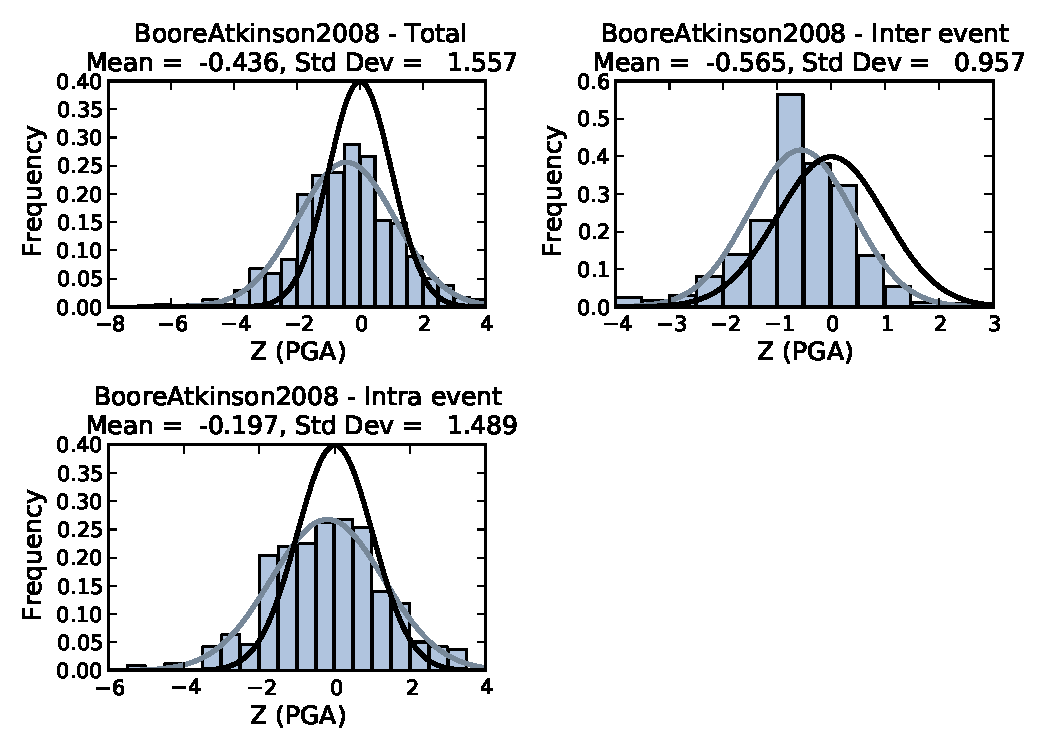
\includegraphics[width=\textwidth]{./figures/residuals/BA2008_Residuals_PGA.pdf}
      \caption{\textcite{boore2008} model}
      \label{fig:pga_res_ba2008}
  \end{subfigure}
    \begin{subfigure}[b]{0.49\textwidth}
      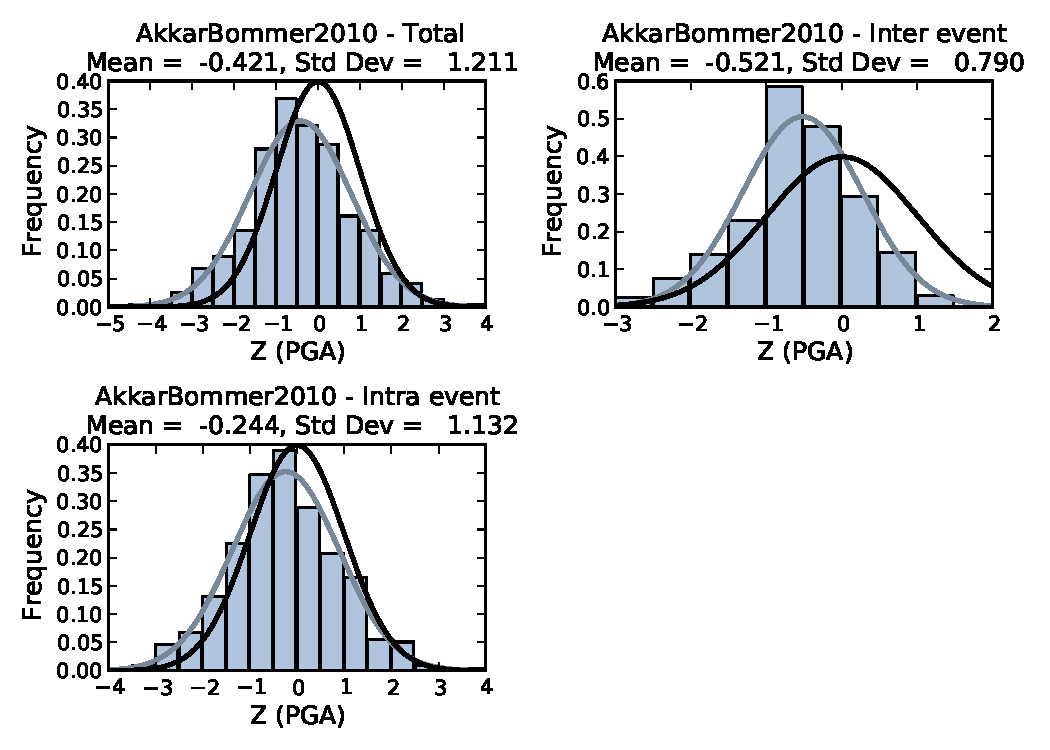
\includegraphics[width=\textwidth]{./figures/residuals/AB2010_Residuals_PGA.pdf}
      \caption{\textcite{AkkarBommer2010} model}
      \label{fig:pga_res_ab2010}
  \end{subfigure}
    \begin{subfigure}[b]{0.49\textwidth}
      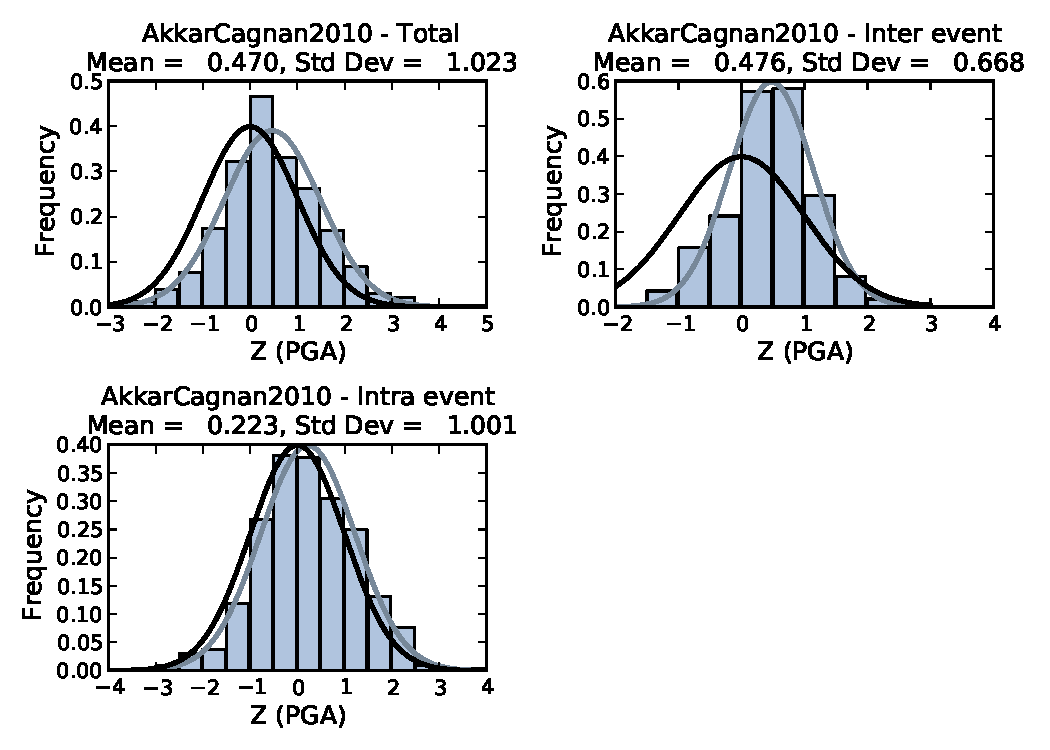
\includegraphics[width=\textwidth]{./figures/residuals/AC2010_Residuals_PGA.pdf}
      \caption{\textcite{AkkarCagnan2010} model}
      \label{fig:pga_res_ac2010}
  \end{subfigure}
      \begin{subfigure}[b]{0.49\textwidth}
      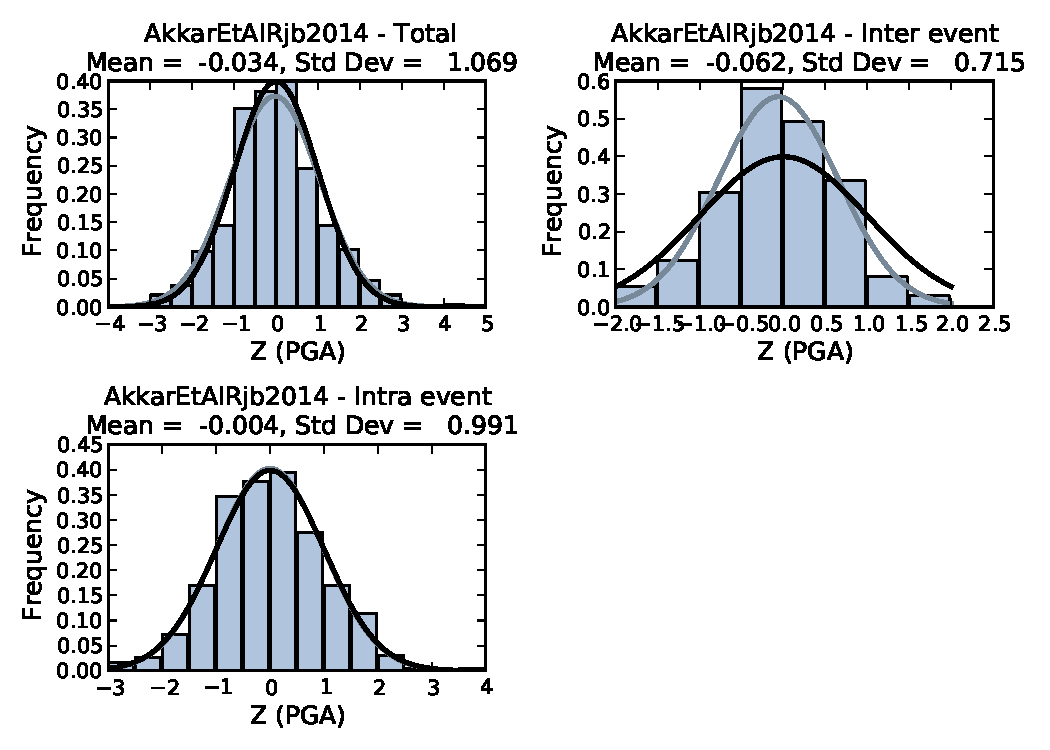
\includegraphics[width=\textwidth]{./figures/residuals/Akkar2014_Residuals_PGA.pdf}
     \caption{\textcite{Akkar_etal2014}model}
      \label{fig:pga_res_akkar2014}
  \end{subfigure}
  \caption{PGA residual distribution for the record set. The grey line indicates the probability density function fit to the data, whilst the black line indicates the standard normal density function}
  \label{fig:pga_resids}
\end{figure}

\begin{figure}[htb]
	\centering
		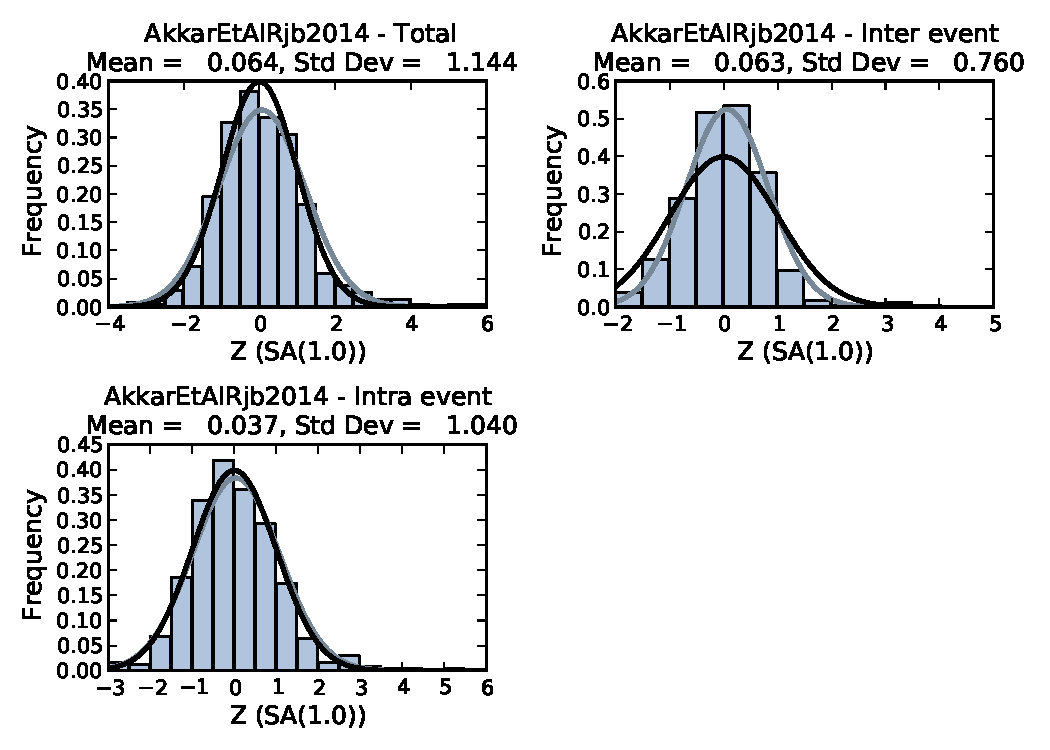
\includegraphics[width=0.6\textwidth]{./figures/residuals/Akkar2014_Residuals_Sa1.pdf}
	\caption{PGA residual distribution for the record set using the \textcite{Akkar_etal2014} GMPE}
	\label{fig:sa1_res_akkar2014}
\end{figure}

Figures \ref{fig:pga_resids} and \ref{fig:sa1_res_akkar2014} shows a relatively discernible set of trends. Consider just the \textcite{boore2008} model for PGA (Figure \ref{fig:pga_res_ba2008}). Each of the residuals have a mean less than zero, significantly so in the case of the inter-event residual. This indicates that in general the \textcite{boore2008} model is predicts higher ground motions than those observed in the records and most of this can be attributed to the inter-event term. The distributions also show a greater spread than expected from the model, as demonstrated by the standard deviation greater than unity. In this case it is the intra-event residuals that show a greater spread than expected, whilst spread in the inter-event residuals is in better agreement with the model. In contrast the \textcite{Akkar_etal2014} GMPE (from which the current records form part of the generating data set) show a much closer agreement with the records (as expected). It is seen that that the distribution of the normalised total residuals is very close to the standard normal distribution; a trend that is matched in the intra-event residuals. Similarly in the inter-event residuals the mean value is close to zero, and only the spread of the model shows a difference, in this case showing a smaller variance than expected from the model. This is to be expected as the current dataset is based on exclusively Italian records (predominantly extensional events, with only a few thrust or oblique slip records), whereas the GMPE was fit to a full set of European and Middle Eastern records, thus incorporating a greater variability of mechanism types than just the Italian subset. The same trend can be seen in the residuals for $Sa \left( {1.0 s} \right)$. 

\section{The Likelihood Model \parencite{Scherbaum_etal2004}}
\label{sec:lh_model}

The basic residual trends can help understand where biases may be present in the model with respect to the record set, but they do not necessarily provide a quantitative indication of the total fit of the model to the record. One possibility to do this (others will presented later in the chapter) is to consider the overall goodness-of-fit of the model to the predictions. \textcite{Scherbaum_etal2004} consider the probability that the absolute value of a random sample from the normalised distribution to fall into the interval between the modulus of a particular observation $|z_0|$ and infinity.

\begin{equation}
u \left( {z_0} \right) = \frac{1}{2} Erf\left( {\frac{z_0}{\sqrt{2}}, \infty} \right)
\end{equation}

The total ``likelihood'' of a particular value is given by:

\begin{equation}
LH \left( {|z_0|} \right) = 2 \cdot u \left( {|z_0|} \right) = Erf \left( {\frac{|z_0|}{\sqrt{2}}, \infty} \right)
\end{equation}

As indicated in \textcite{Scherbaum_etal2004} the the $LH$ value should reach a value of $1$ for $|z_0|=0$ (i.e. the mean of the distribution), and should tend to zero for observations further away from the mean. Therefore, if the model assumptions are matched exactly by a set of observations then the $LH \left( {|z_0|} \right)$ values should be distributed evenly between 0 and 1, with a median value of 0.5. 

The GMPE-SMTK can produce histograms of the $LH$ value for the ground motion observations using the \verb=res.Likelihood= and \verb=rspl.LikelihoodPlot= tools. The \verb=res.Likeihood= tool operates in the same manner as the \verb=res.Residuals= tool; therefore to run the likelihood analysis one follows the same approach:

\begin{python}[frame=single]
# Set-up the likelihood calculator
lh1 = res.Likelihood(gmpe_list, imts)
# Run the residual calculator
lh1.get_residuals(sm_database)
\end{python}

Histograms of the $LH$ values (and their median estimates) for the four GMPEs for PGA are shown in Figure \ref{fig:pga_lh}, and for only \textcite{Akkar_etal2014} for $Sa \left( {1.0 s} \right)$ in Figure \ref{fig:sa1_lh_akkar2014} . These can be generated with the following command:

\begin{python}
# Boore & Atkinson (2008)
rspl.LikelihoodPlot(lh1, "BooreAtkinson2008", "PGA",
                    filename="path/to/image.png",
                    filetype="png")
# Akkar & Bommer (2010)
rspl.LikelihoodPlot(lh1, "AkkarBommer2010", "PGA")
# Akkar & Cagnan (2010)
rspl.LikelihoodPlot(lh1, "AkkarCagnan2010", "PGA")
# Akker et al. (2014)
rspl.LikelihoodPlot(lh1, "AkkarEtAlRjb2014", "PGA")
# Akker et al. (2014) - Sa (1.0 s)
rspl.LikelihoodPlot(lh1, "AkkarEtAlRjb2014", "Sa(1.0)")
\end{python}

\begin{figure}[htb]
  \centering
  \begin{subfigure}[b]{0.49\textwidth}
      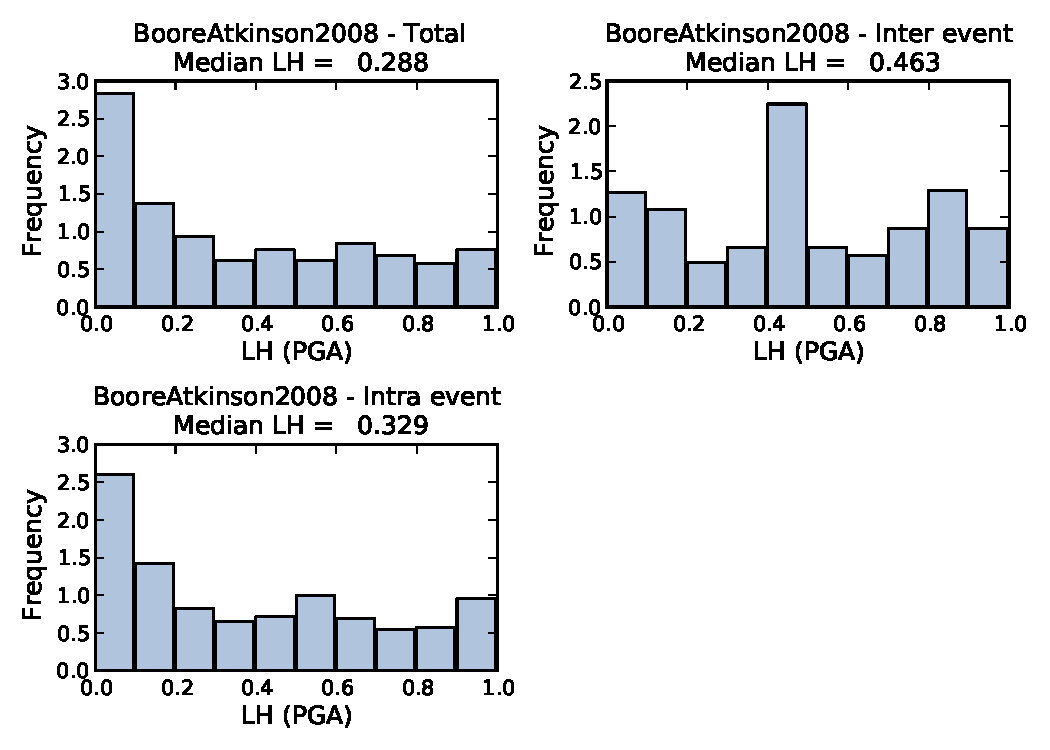
\includegraphics[width=\textwidth]{./figures/residuals/BA2008_LH_PGA.pdf}
      \caption{\textcite{boore2008} model}
      \label{fig:pga_lh_ba2008}
  \end{subfigure}
    \begin{subfigure}[b]{0.49\textwidth}
      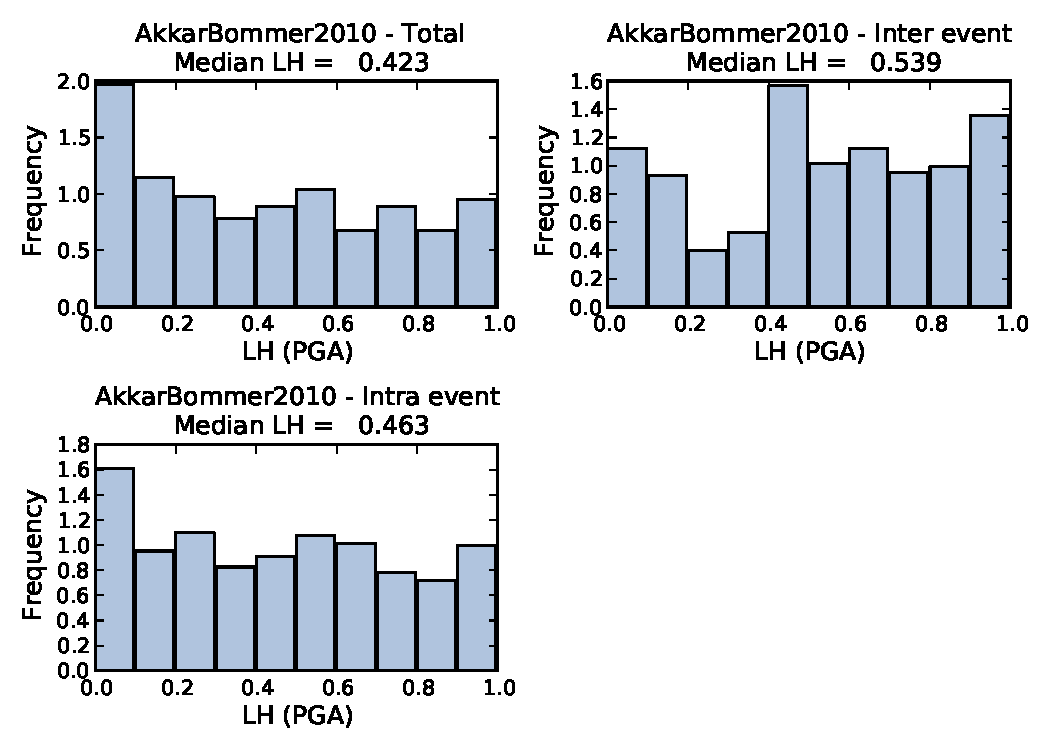
\includegraphics[width=\textwidth]{./figures/residuals/AB2010_LH_PGA.pdf}
      \caption{\textcite{AkkarBommer2010} model}
      \label{fig:pga_lh_ab2010}
  \end{subfigure}
    \begin{subfigure}[b]{0.49\textwidth}
      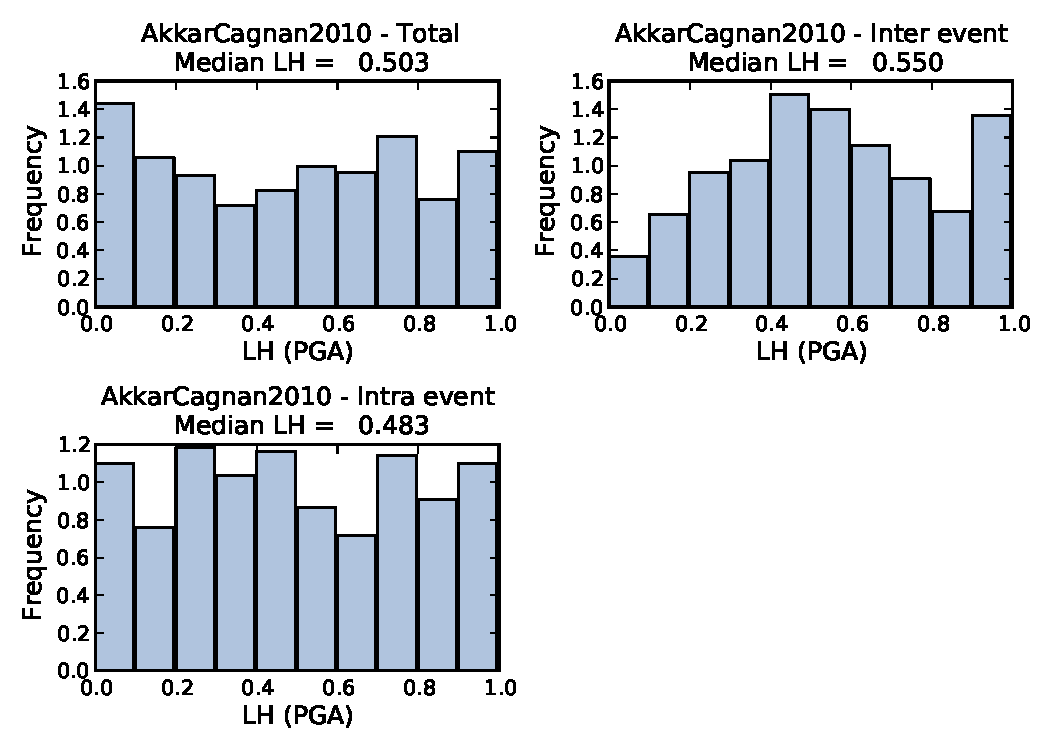
\includegraphics[width=\textwidth]{./figures/residuals/AC2010_LH_PGA.pdf}
      \caption{\textcite{AkkarCagnan2010} model}
      \label{fig:pga_lh_ac2010}
  \end{subfigure}
      \begin{subfigure}[b]{0.49\textwidth}
      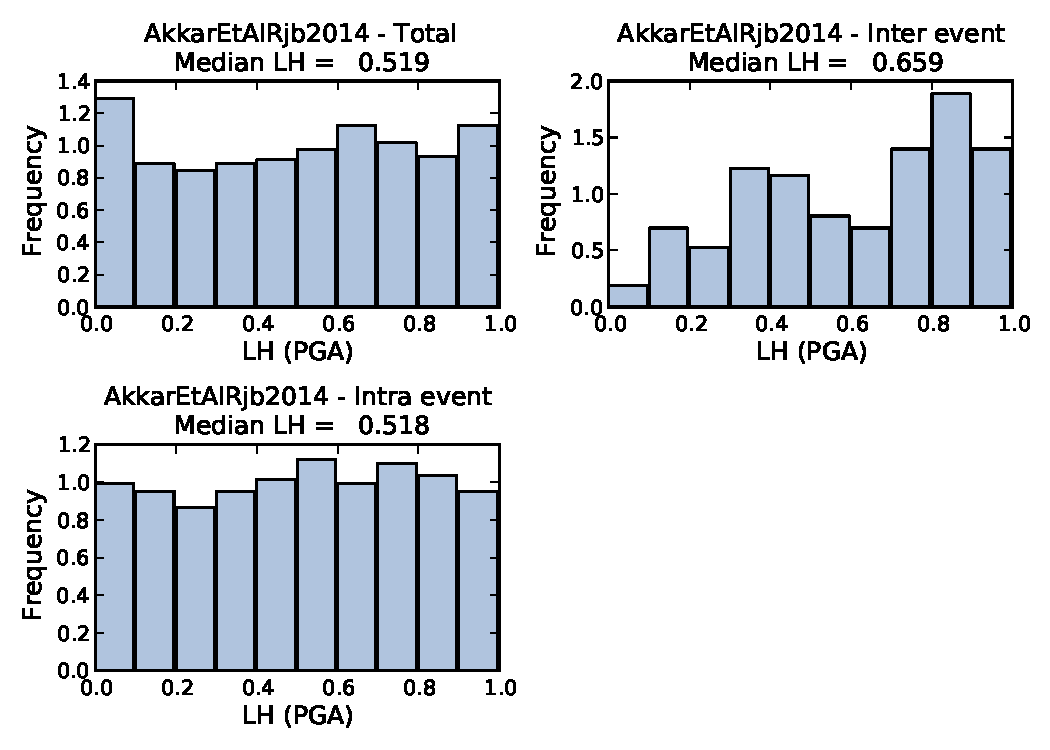
\includegraphics[width=\textwidth]{./figures/residuals/Akkar2014_LH_PGA.pdf}
     \caption{\textcite{Akkar_etal2014} model}
      \label{fig:pga_lh_akkar2014}
  \end{subfigure}
  \caption{$LH$ distribution for the observed PGA set}
  \label{fig:pga_lh}
\end{figure}

\begin{figure}[htb]
	\centering
		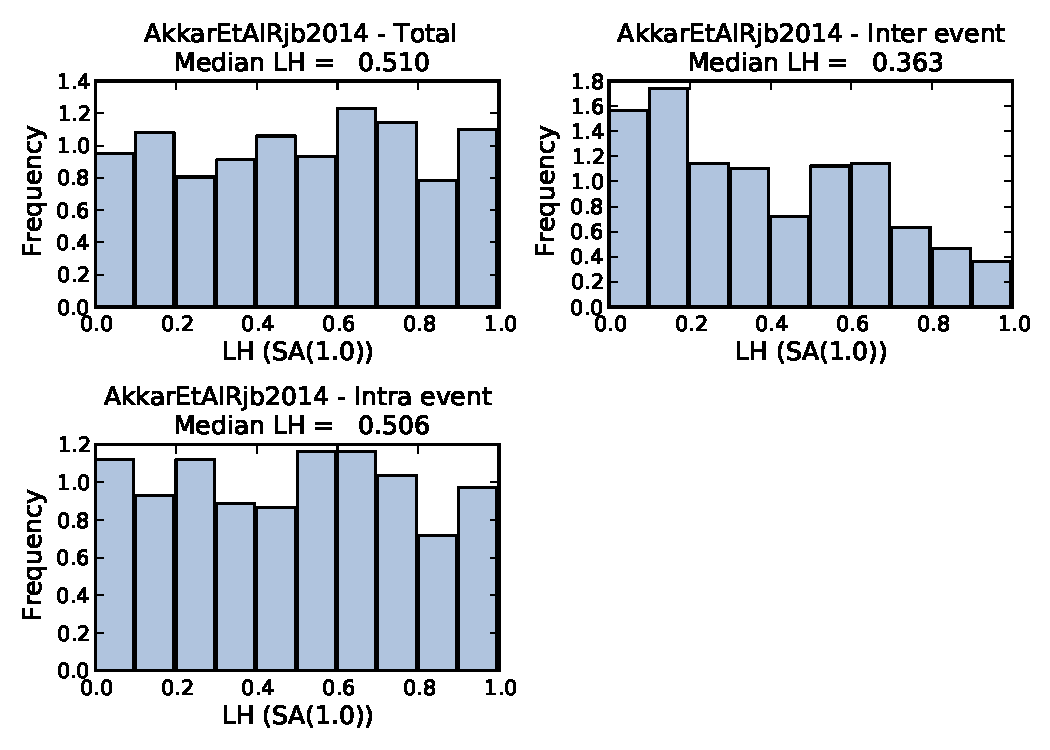
\includegraphics[width=0.6\textwidth]{./figures/residuals/Akkar2014_LH_Sa1.pdf}
	\caption{$LH$ distribution for the observed $Sa \left( {1.0 s} \right)$ set using the \textcite{Akkar_etal2014} GMPE}
	\label{fig:sa1_lh_akkar2014}
\end{figure}

In general the trends seen in Figure \ref{fig:pga_resids} are visible in the $LH$ histograms in the manner described in \textcite{Scherbaum_etal2004}. In the \textcite{boore2008} model intra-event and total residuals showed a greater variance than predicted by the GMPE, a trend that tends to result in $LH$ values closer to zero than 1. For the \textcite{Akkar_etal2014} GMPE both the total and inter-event residuals are generally evenly distributed between 0 and 1, with a median of close to 0.5, indicating a good agreement between the model and observations. The inter-event residuals show a smaller range than that expected by the model and so the $LH$ values are closer to 1.0 (the distances from the mean are smaller than expected). 

\section{Residual Trends with Predictor Variables}
\label{sec:predictor_trends}

The analysis of the residuals shown in sections \ref{sec:residual_trends} and \ref{sec:lh_model} provide useful insights into the overall fit of a GMPE to a set of observations. They do not necessarily provide a clear indication as to which elements of the model contribute to the misfit. Or, to frame it differently, they do not necessarily indicate where the GMPEs may be biased with respect to the predictor variables of the observations. To analysis this it is necessary to understand if, and where, the GMPE residuals show clear trends with respect to the predictor variables. These trends can indicate those elements of the source/site scaling and attenuation process for which the GMPE is biased.

The GMPE-SMTK offers several methods to visualise the trends of the GMPE residuals with the following predictor variables:
\begin{enumerate}
\item Magnitude
\item Distance
\item $V_{S30}$
\item Hypocentral Depth
\end{enumerate}

\subsubsection{Trends with Magnitude}

To view the trends with magnitude for a set of ground motion residuals the \verb=rspl= toolset contains the function \verb=ResidualWithMagnitude=. Figure \ref{fig:mag_resid} shows the residual trends in magnitude for the \textcite{boore2008} and \textcite{Akkar_etal2014} GMPEs for PGA and $Sa \left( {1.0 s} \right)$. These figures were generated with the following commands:

\begin{python}[frame=single]
# Boore & Atkinson (2008)  - PGA
rspl.ResidualWithMagnitude(resid1,  # Residuals
                           "BooreAtkinson2008",  # GMPE
                           "PGA",   # Intensity Measure
                           filename="path/to/image.png",
                           filetype="png")
# Akkar et al. (2014)  - PGA
rspl.ResidualWithMagnitude(resid1, "AkkarEtAlRjb2014", "PGA") 
# Boore & Atkinson (2008)  - Sa (1.0)
rspl.ResidualWithMagnitude(resid1, "BooreAtkinson2008",
                          "Sa(1.0)") 
# Akkar et al. (2014)  - Sa (1.0)
rspl.ResidualWithMagnitude(resid1, "AkkarEtAlRjb2014",
                          "Sa(1.0)")                         
\end{python}

As shown in Figure \ref{fig:mag_resid}, and in subsequent figures, a linear model is fit to the observed residual trends. The significance of the trend is measured via the ``p-value'', reported in the figure header. This indicates the probability observing the measured trend in the residuals assuming a null hypothesis of no trend (i.e. zero gradient). Consequently a smaller ``p-value'' indicates a more significant trend, assuming (loosely) that statistically significant trends might be those with a ``p-value'' smaller than 0.1. If the magnitude scaling is largely unbiased with respect to the GMPE it is expected that no significant linear trend can be observed the plot of residuals with magnitude. This is the case for the \textcite{Akkar_etal2014} GMPE in which no statistically significant trend is observed with respect to magnitude. For the \textcite{boore2008} model a statistically significant trend is visible in the inter-event residuals. For PGA this trend is negative, suggesting that the GMPE is predicting higher than observed ground motions for the larget magnitudes, whilst for $Sa \left( {1.0 s} \right)$ the opposite is true, indicating the GMPE is predicting lower than expected ground motions at higher magnitudes.

\begin{figure}[htb]
  \centering
  \begin{subfigure}[b]{0.49\textwidth}
      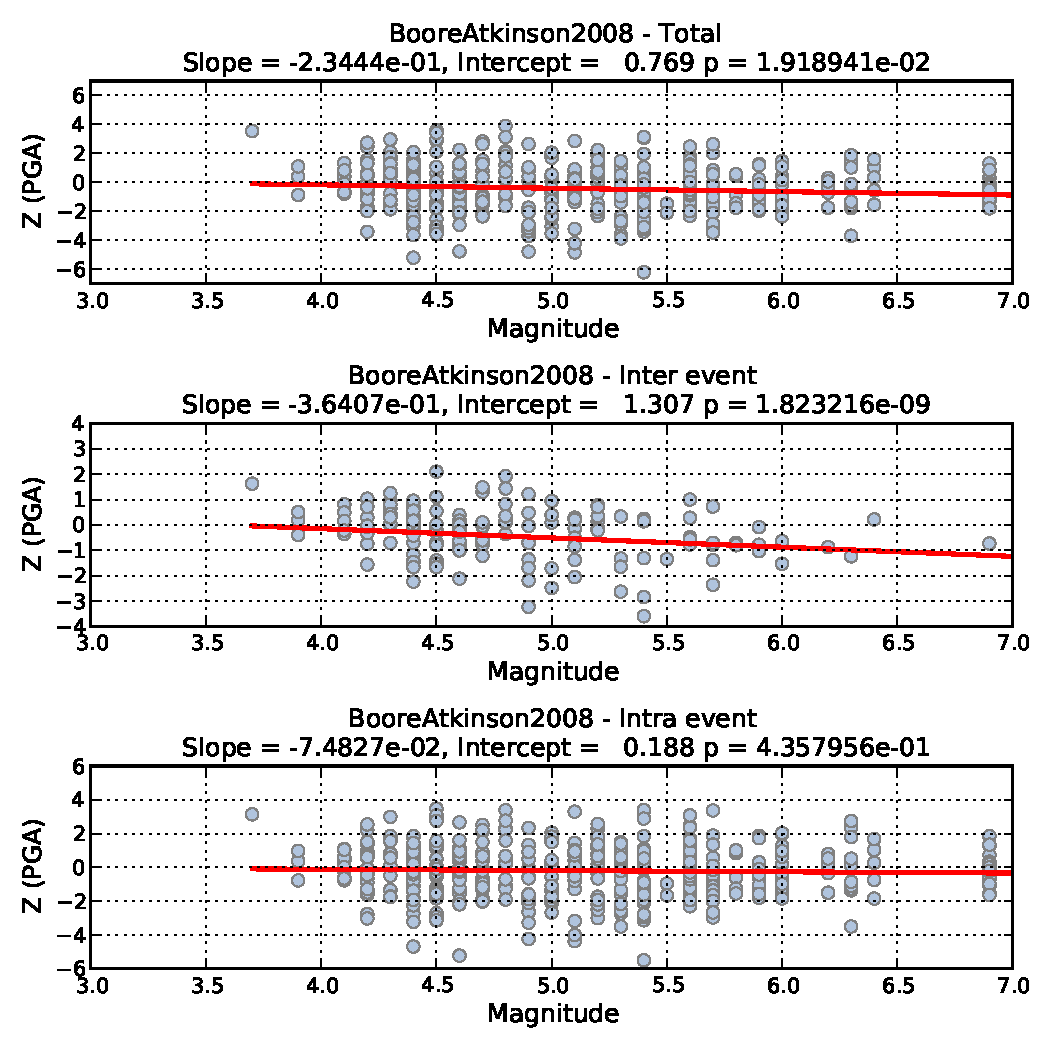
\includegraphics[width=\textwidth]{./figures/residuals/BA2008_Magnitude_PGA.pdf}
      \caption{\textcite{boore2008} model - PGA}
      \label{fig:pga_mag_ba2008}
  \end{subfigure}
    \begin{subfigure}[b]{0.49\textwidth}
      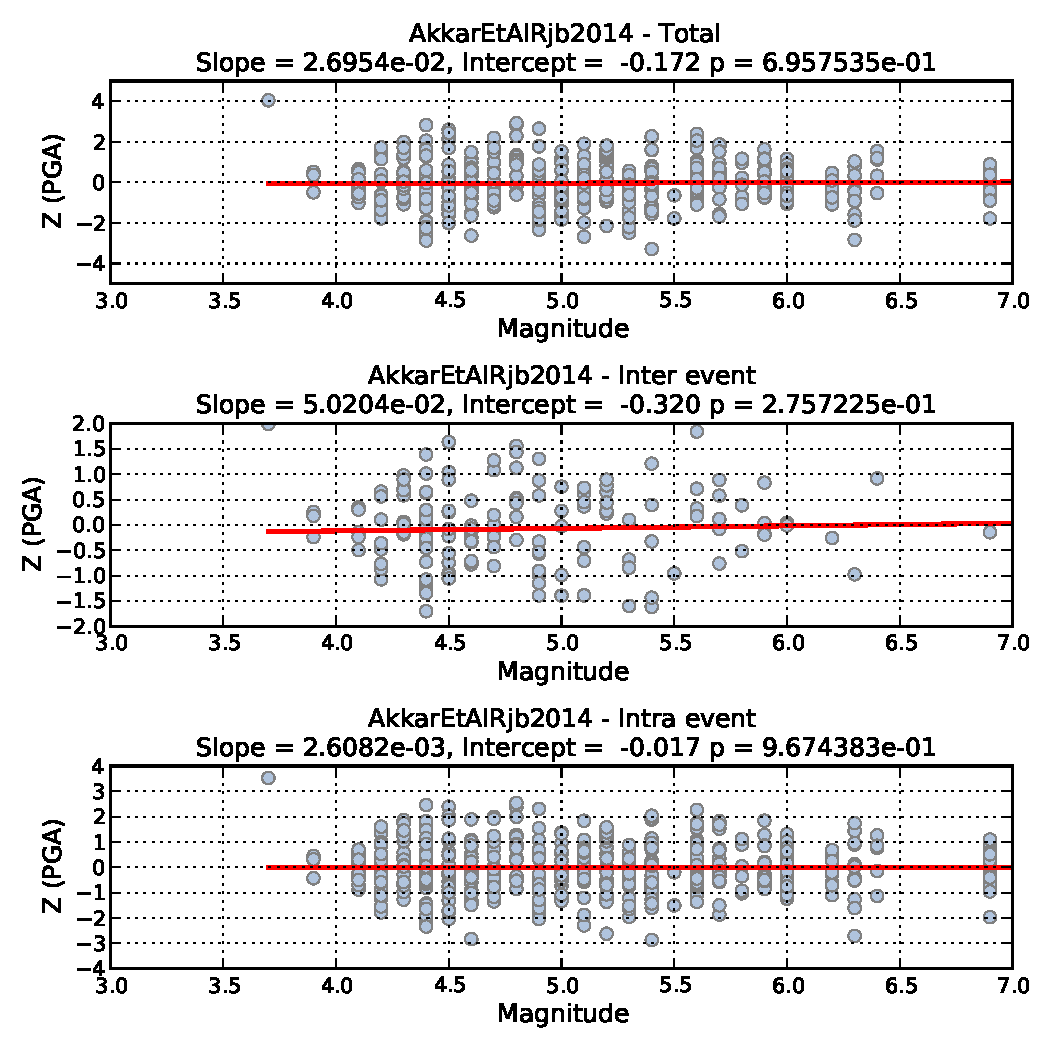
\includegraphics[width=\textwidth]{./figures/residuals/Akkar2014_Magnitude_PGA.pdf}
      \caption{\textcite{Akkar_etal2014} model - PGA}
      \label{fig:pga_mag_akkar2014}
  \end{subfigure}
    \begin{subfigure}[b]{0.49\textwidth}
      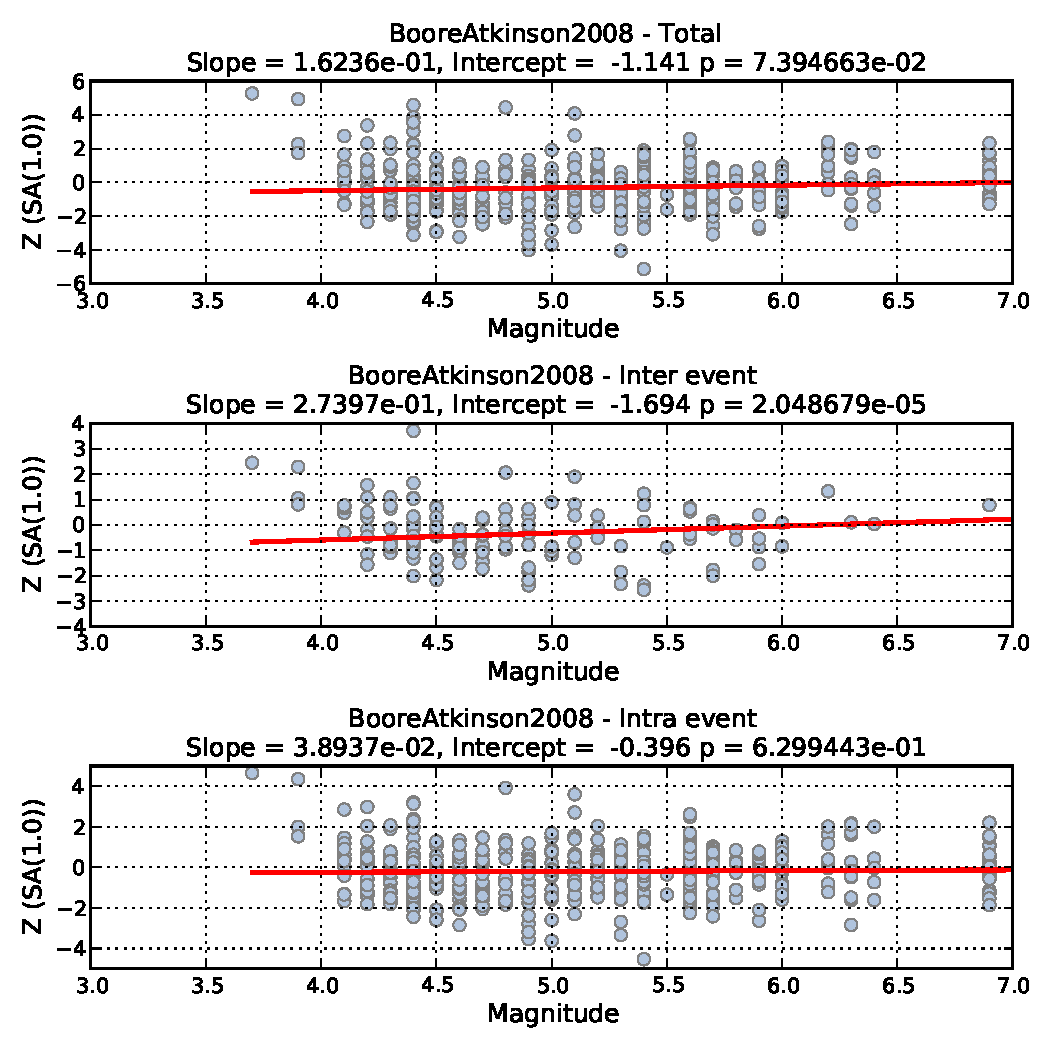
\includegraphics[width=\textwidth]{./figures/residuals/BA2008_Magnitude_Sa1.pdf}
      \caption{\textcite{boore2008} model - $Sa \left( {1.0 s} \right)$}
      \label{fig:sa1_mag_ba2008}
  \end{subfigure}
      \begin{subfigure}[b]{0.49\textwidth}
      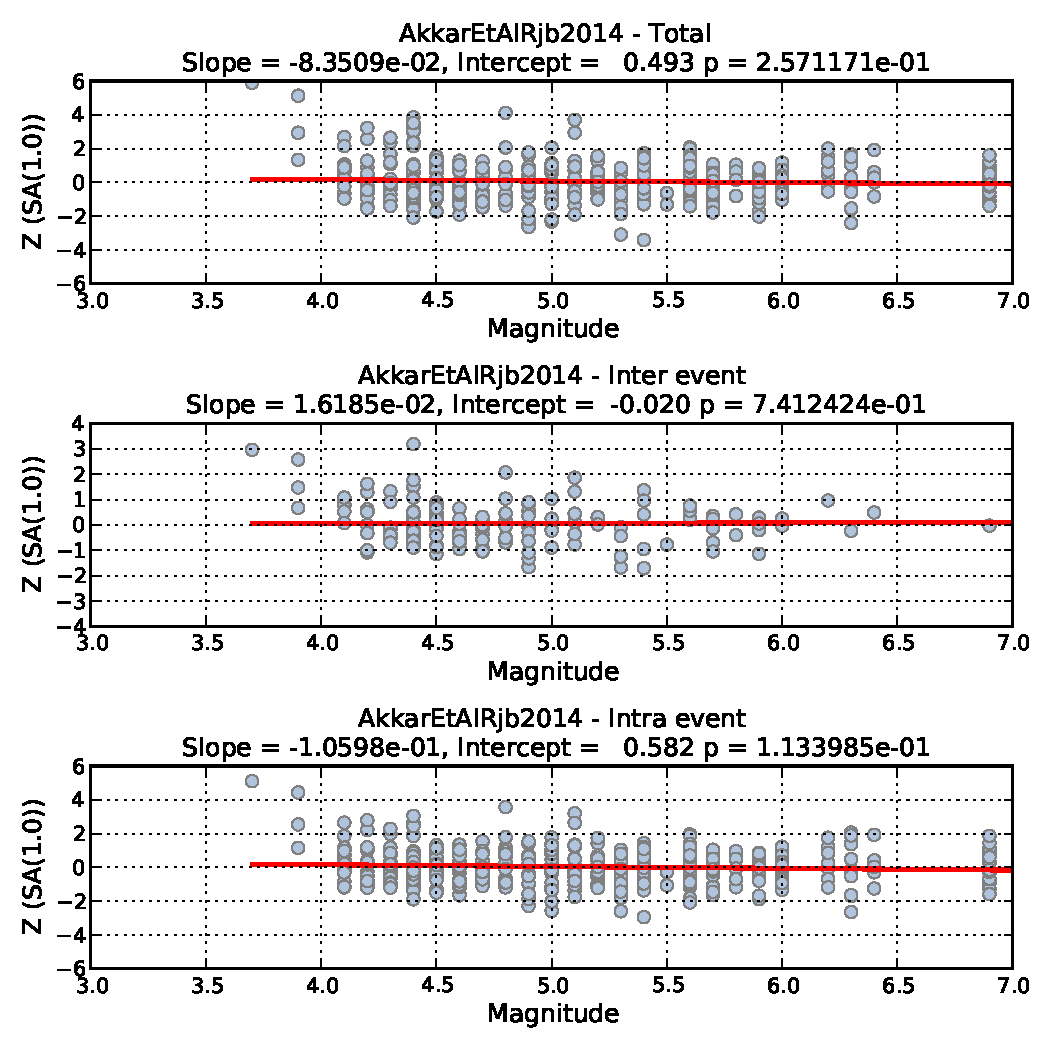
\includegraphics[width=\textwidth]{./figures/residuals/Akkar2014_Magnitude_Sa1.pdf}
     \caption{\textcite{Akkar_etal2014} model - $Sa \left( {1.0 s} \right)$}
      \label{fig:sa1_mag_akkar2014}
  \end{subfigure}
  \caption{Residual trends with magnitude for the observed PGA and $Sa \left( {1.0 s} \right)$ records}
  \label{fig:mag_resid}
\end{figure}


\subsubsection{Trends with Distance}

To observe how well the GMPE compares to the distance attenuation properties in a set of records the \verb=rspl= tools provide the method \verb=ResidualWithDistance=. Plots of residuals with distance for the same GMPEs and intensity measures considered in Figure \ref{fig:mag_resid} are shown in Figure \ref{fig:dist_resid}. These are generated using the following commands:

\begin{python}[frame=single]
# Boore & Atkinson (2008)  - PGA
rspl.ResidualWithDistance(resid1,  # Residuals
                           "BooreAtkinson2008",  # GMPE
                           "PGA",   # Intensity Measure
                           distance_type="rjb"
                           plot_type="linear",
                           filename="path/to/image.png",
                           filetype="png")
# Akkar et al. (2014)  - PGA
rspl.ResidualWithDistance(resid1, "AkkarEtAlRjb2014",
                          "PGA", distance_type="rjb",
                          plot_type="linear") 
# Boore & Atkinson (2008)  - Sa (1.0)
rspl.ResidualWithDistance(resid1, "BooreAtkinson2008",
                          "Sa(1.0)", distance_type="rjb",
                          plot_type="linear") 
# Akkar et al. (2014)  - Sa (1.0)
rspl.ResidualWithDistance(resid1, "AkkarEtAlRjb2014",
                          "Sa(1.0)", distance_type="rjb",
                          plot_type="linear")                         
\end{python}

The input arguments are identical to the \verb=ResidualwithMagnitude= tool, with the exception of the \verb=distance_type= and \verb=plot_type= keywords. The \verb=distance_type= determines the distance measure used for visualisation, whilst the \verb=plot_type= keyword indicates whether to plot the distance values on a logarithmic axis (``\verb=log='') or a linear axis (``\verb=linear=''). A logarithmic axis is preferred by default.

In contrast to the residual trends with magnitude, it is evident in Figure \ref{fig:dist_resid} that statistically significant trends with distance exist for both GMPEs. This can be clearly seen in the intra-event residual, which shows a negative trend in the residuals, a trend that is more pronounced for the \textcite{boore2008} model. This indicates that both models underestimate the degree of attenuation in the ground motions observed in Italy, as both models predict higher ground motion at greater distances than those observed in the strong motion records. 

\begin{figure}[htb]
  \centering
  \begin{subfigure}[b]{0.49\textwidth}
      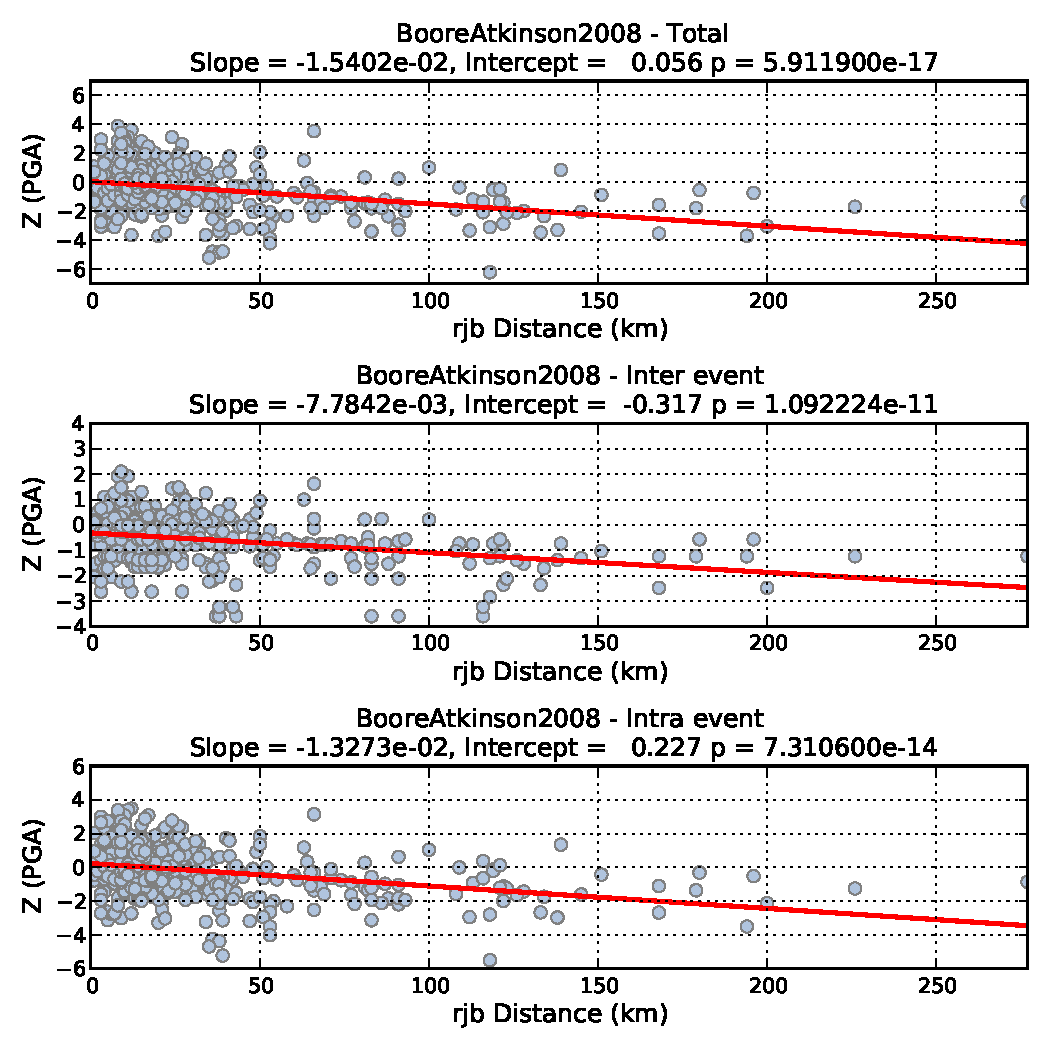
\includegraphics[width=\textwidth]{./figures/residuals/BA2008_Distance_PGA.pdf}
      \caption{\textcite{boore2008} model - PGA}
      \label{fig:pga_dist_ba2008}
  \end{subfigure}
    \begin{subfigure}[b]{0.49\textwidth}
      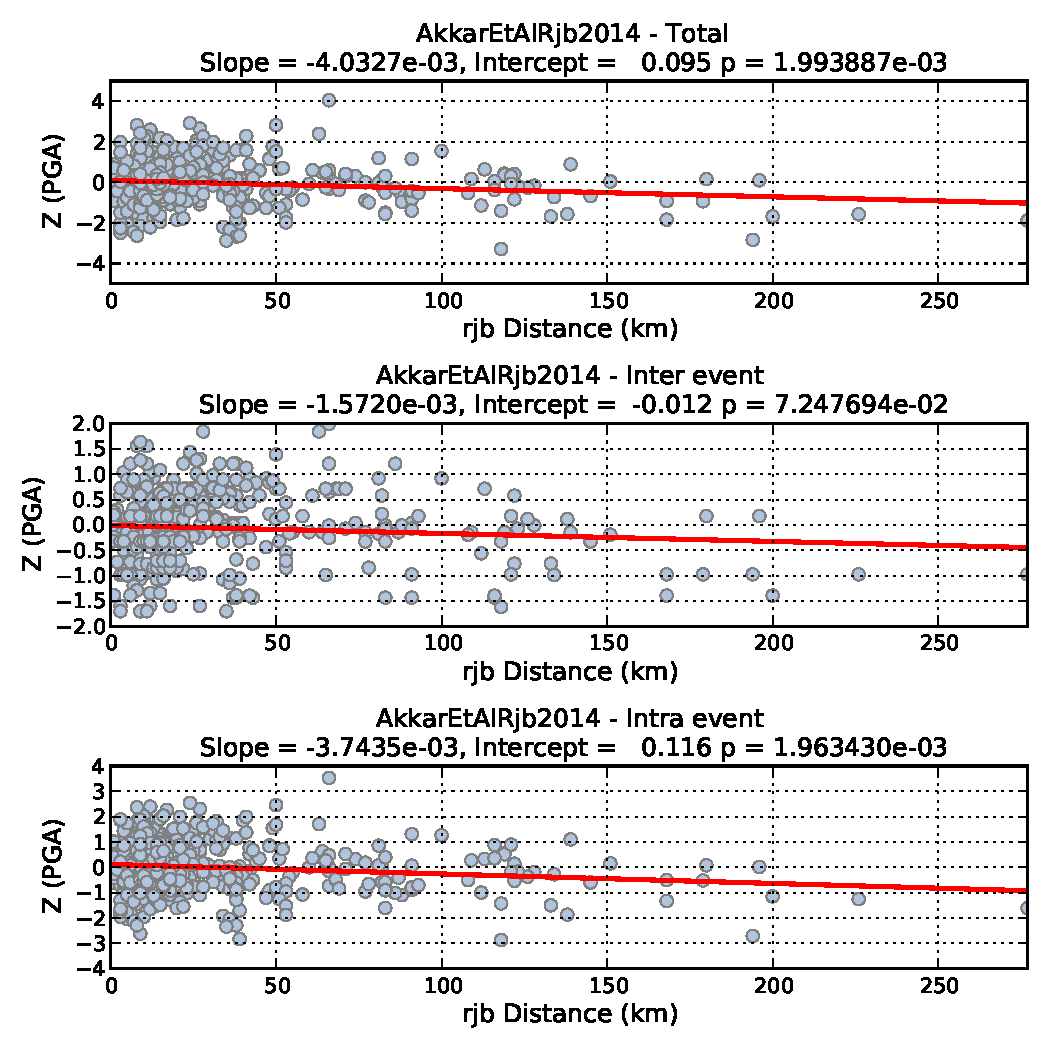
\includegraphics[width=\textwidth]{./figures/residuals/Akkar2014_Distance_PGA.pdf}
      \caption{\textcite{Akkar_etal2014} model - PGA}
      \label{fig:pga_dist_akkar2014}
  \end{subfigure}
    \begin{subfigure}[b]{0.49\textwidth}
      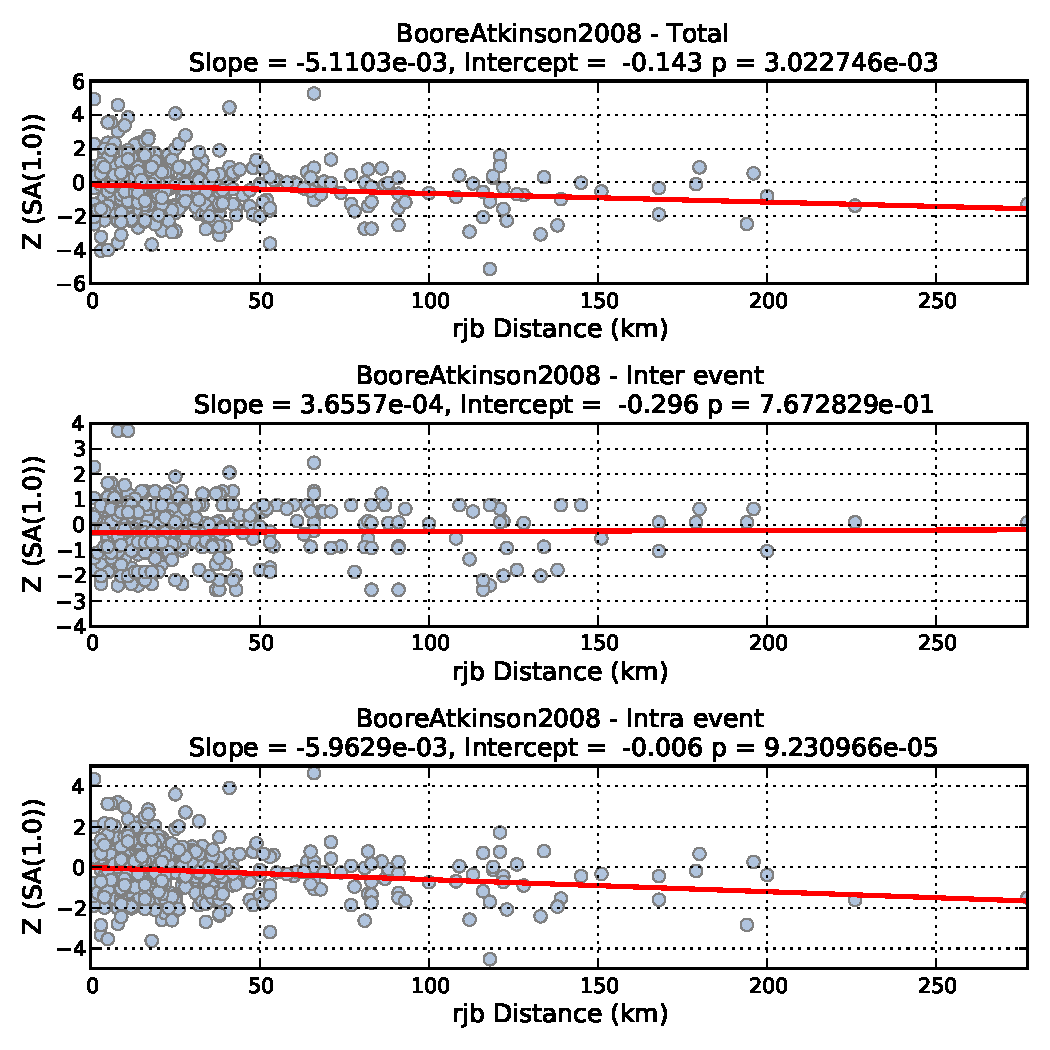
\includegraphics[width=\textwidth]{./figures/residuals/BA2008_Distance_Sa1.pdf}
      \caption{\textcite{boore2008} model - $Sa \left( {1.0 s} \right)$}
      \label{fig:sa1_dist_ba2008}
  \end{subfigure}
      \begin{subfigure}[b]{0.49\textwidth}
      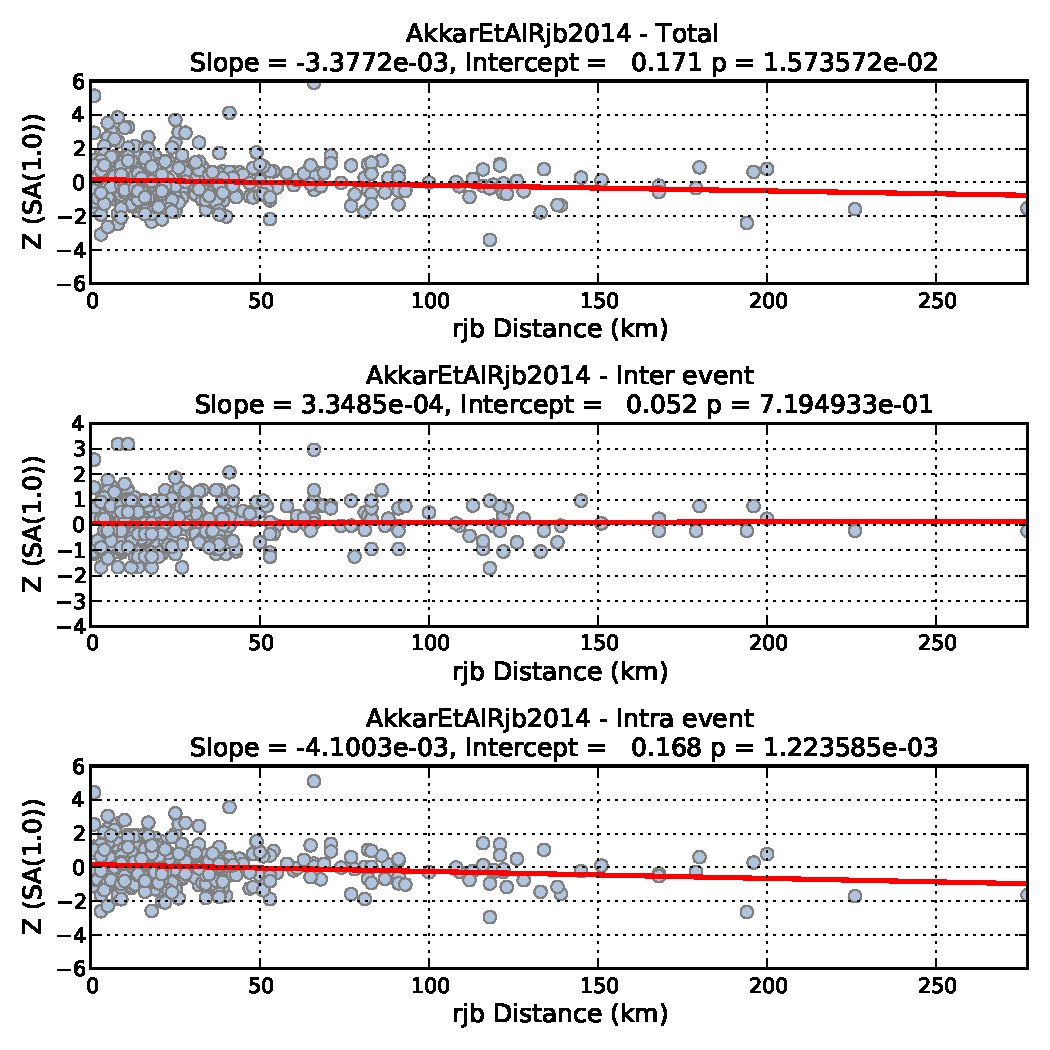
\includegraphics[width=\textwidth]{./figures/residuals/Akkar2014_Distance_Sa1.pdf}
     \caption{\textcite{Akkar_etal2014} model - $Sa \left( {1.0 s} \right)$}
      \label{fig:sa1_dist_akkar2014}
  \end{subfigure}
  \caption{Residual trends with Joyner-Boore distance for the observed PGA and $Sa \left( {1.0 s} \right)$ records}
  \label{fig:dist_resid}
\end{figure}

\subsubsection{Trends with $V_{S30}$}

The usage of the \verb=rspl= tool to visualise residual trends with $V_{S30}$ (\verb=ResidualWithVs30=) is generally the same as the tools for the magnitude and distance. So for the same GMPEs and intensity measures considered previously, the following commands are used to produce the plot of residuals against $V_{S30}$ for the same record set, shown in Figure \ref{fig:vs30_resid}:
 
 \begin{python}[frame=single]
# Boore & Atkinson (2008)  - PGA
rspl.ResidualWithVs30(resid1,  # Residuals
                      "BooreAtkinson2008",  # GMPE
                      "PGA",   # Intensity Measure
                      filename="path/to/image.png",
                      filetype="png")
# Akkar et al. (2014)  - PGA
rspl.ResidualWithVs30(resid1, "AkkarEtAlRjb2014", "PGA") 
# Boore & Atkinson (2008)  - Sa (1.0)
rspl.ResidualWithVs30(resid1, "BooreAtkinson2008", "Sa(1.0)") 
# Akkar et al. (2014)  - Sa (1.0)
rspl.ResidualWithVs30(resid1, "AkkarEtAlRjb2014", "Sa(1.0)")                         
\end{python}

Once again in both the GMPEs and for both intensity measures there are statistically significant trends in the residuals with $V_{S30}$. In most cases the trends are positive, with a negative intercept, indicating that the GMPEs are predicting higher than expected ground motions on softer soils (i.e. lower $V_{s30}$) for the selected stations.

\begin{figure}[htb]
  \centering
  \begin{subfigure}[b]{0.49\textwidth}
      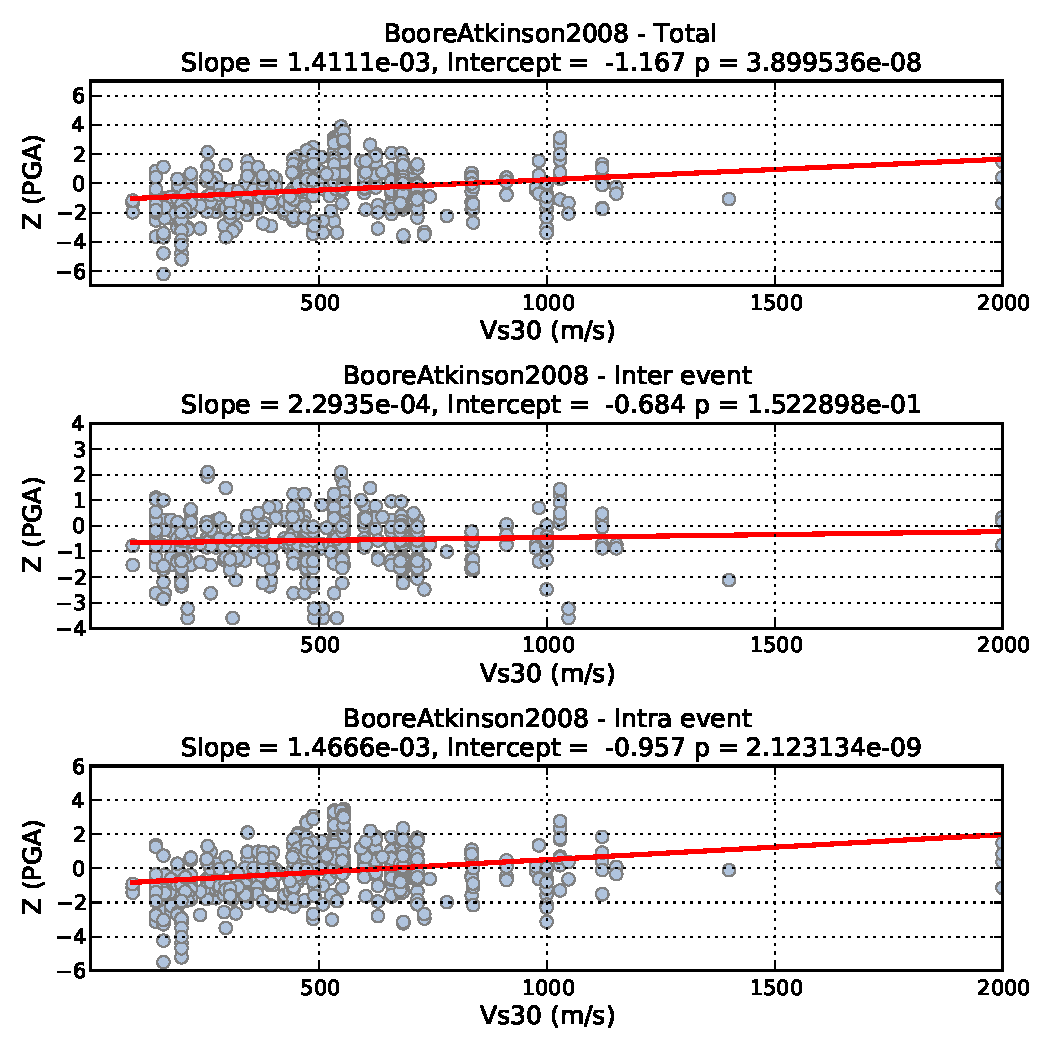
\includegraphics[width=\textwidth]{./figures/residuals/BA2008_Vs30_PGA.pdf}
      \caption{\textcite{boore2008} model - PGA}
      \label{fig:pga_vs30_ba2008}
  \end{subfigure}
    \begin{subfigure}[b]{0.49\textwidth}
      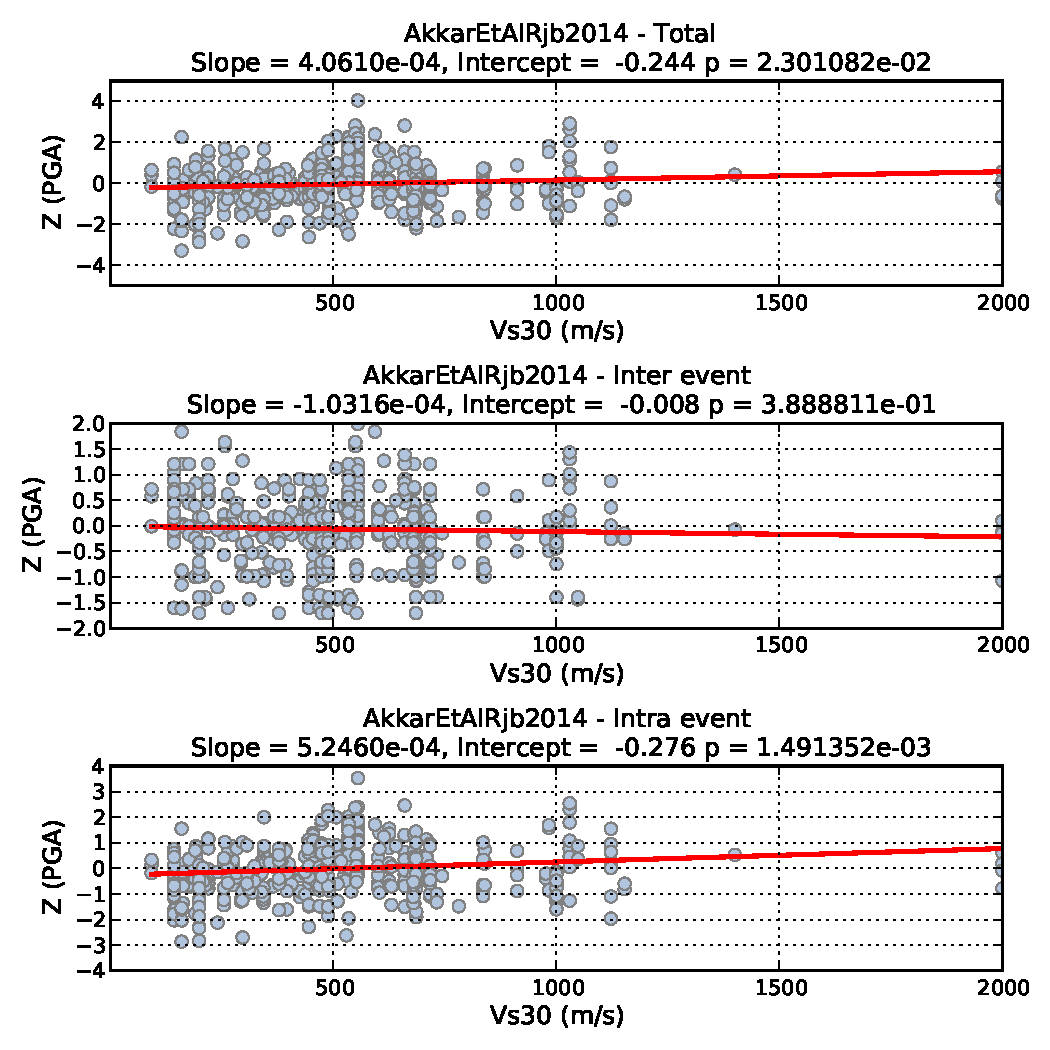
\includegraphics[width=\textwidth]{./figures/residuals/Akkar2014_Vs30_PGA.pdf}
      \caption{\textcite{Akkar_etal2014} model - PGA}
      \label{fig:pga_vs30_akkar2014}
  \end{subfigure}
    \begin{subfigure}[b]{0.49\textwidth}
      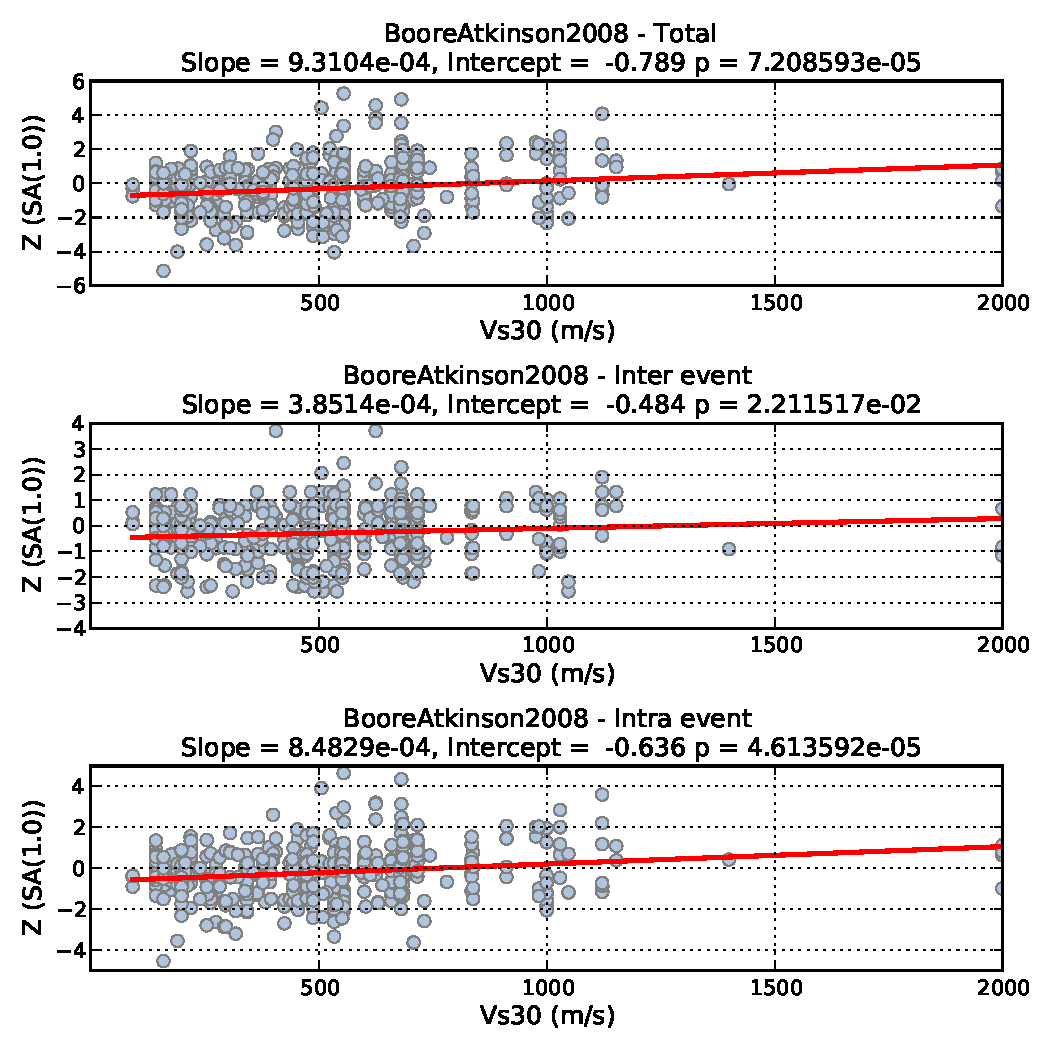
\includegraphics[width=\textwidth]{./figures/residuals/BA2008_Vs30_Sa1.pdf}
      \caption{\textcite{boore2008} model - $Sa \left( {1.0 s} \right)$}
      \label{fig:sa1_vs30_ba2008}
  \end{subfigure}
      \begin{subfigure}[b]{0.49\textwidth}
      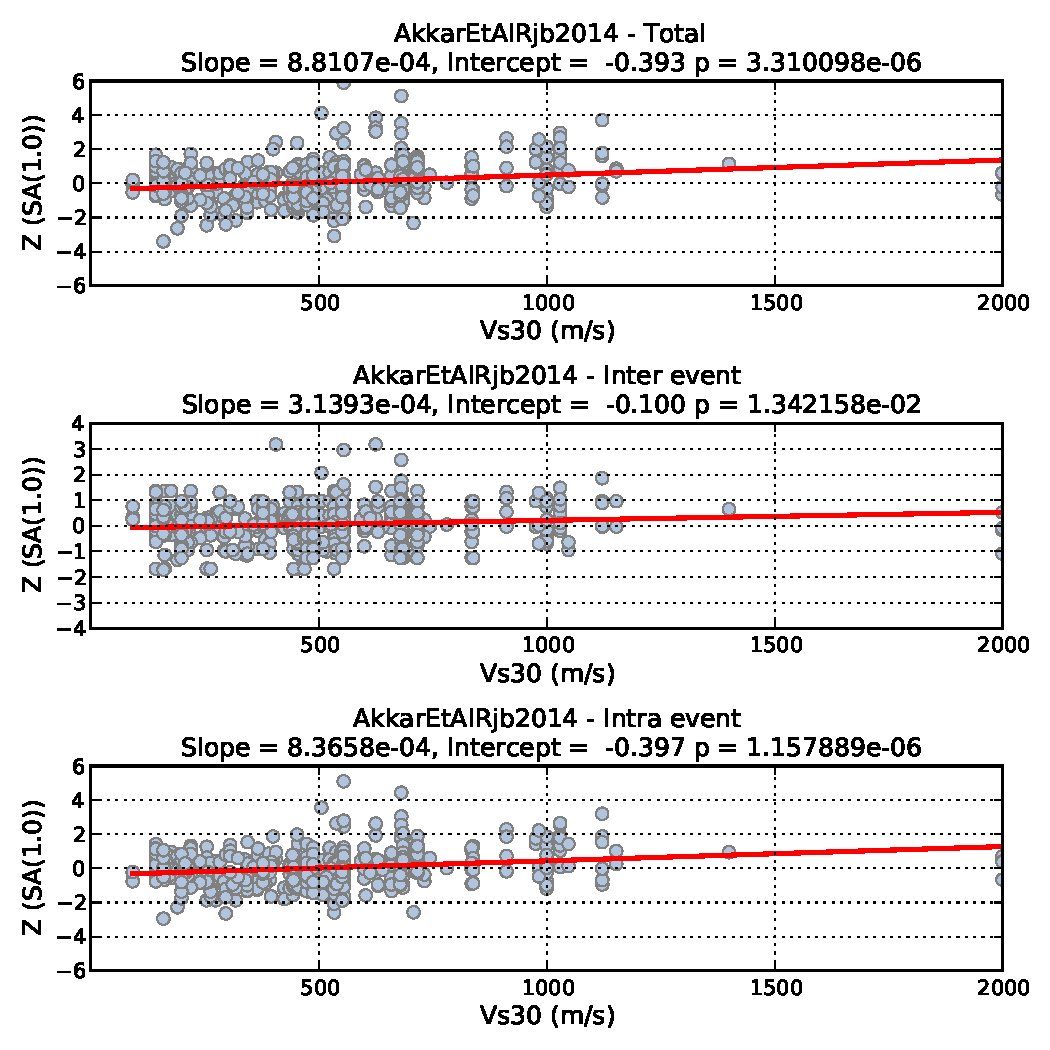
\includegraphics[width=\textwidth]{./figures/residuals/Akkar2014_Vs30_Sa1.pdf}
     \caption{\textcite{Akkar_etal2014} model - $Sa \left( {1.0 s} \right)$}
      \label{fig:sa1_vs30_akkar2014}
  \end{subfigure}
  \caption{Residual trends with $V_{S30}$ for the observed PGA and $Sa \left( {1.0 s} \right)$ records}
  \label{fig:vs30_resid}
\end{figure}

\subsubsection{Trends with Hypocentral Depth}

Finally, the \verb=rspl= tools contain the method \verb=ResidualWithDepth= to show the trend in the GMPE residuals with \emph{hypocentral} depth. As with the previous residual plotting tools, the commands below will produce plots similar to those shown in Figure \ref{fig:depth_resid}:

 \begin{python}[frame=single]
# Boore & Atkinson (2008)  - PGA
rspl.ResidualWithDepth(resid1,  # Residuals
                      "BooreAtkinson2008",  # GMPE
                      "PGA",   # Intensity Measure
                      filename="path/to/image.png",
                      filetype="png")
# Akkar et al. (2014)  - PGA
rspl.ResidualWithDepth(resid1, "AkkarEtAlRjb2014", "PGA") 
# Boore & Atkinson (2008)  - Sa (1.0)
rspl.ResidualWithDepth(resid1, "BooreAtkinson2008", "Sa(1.0)") 
# Akkar et al. (2014)  - Sa (1.0)
rspl.ResidualWithDepth(resid1, "AkkarEtAlRjb2014", "Sa(1.0)")                         
\end{python}

In this case both GMPEs show statistically significant negative trends in the residual with respect to depth. As expected, it is the inter-event residual where these trends are evident, and that control the trends in the total residual. This indicates that the GMPEs are predicting higher ground motions for deeper events than those observed. For the two GMPEs considered, this result is somewhat expected as neither have an explicit dependence on a depth predictor variable; hence hypocentral depth is within the aleatory variability of the model. 

\begin{figure}[htb]
  \centering
  \begin{subfigure}[b]{0.49\textwidth}
      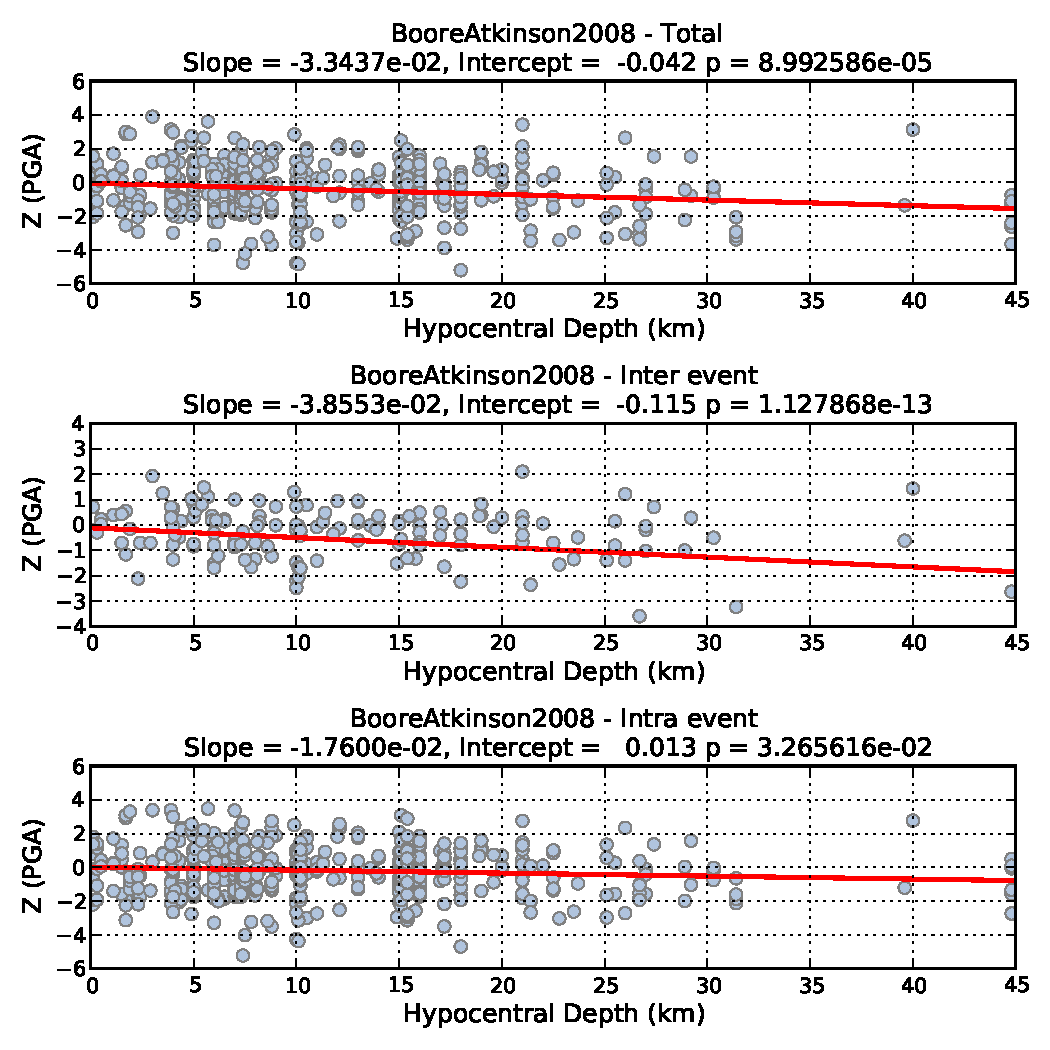
\includegraphics[width=\textwidth]{./figures/residuals/BA2008_HypoDepth_PGA.pdf}
      \caption{\textcite{boore2008} model - PGA}
      \label{fig:pga_depth_ba2008}
  \end{subfigure}
    \begin{subfigure}[b]{0.49\textwidth}
      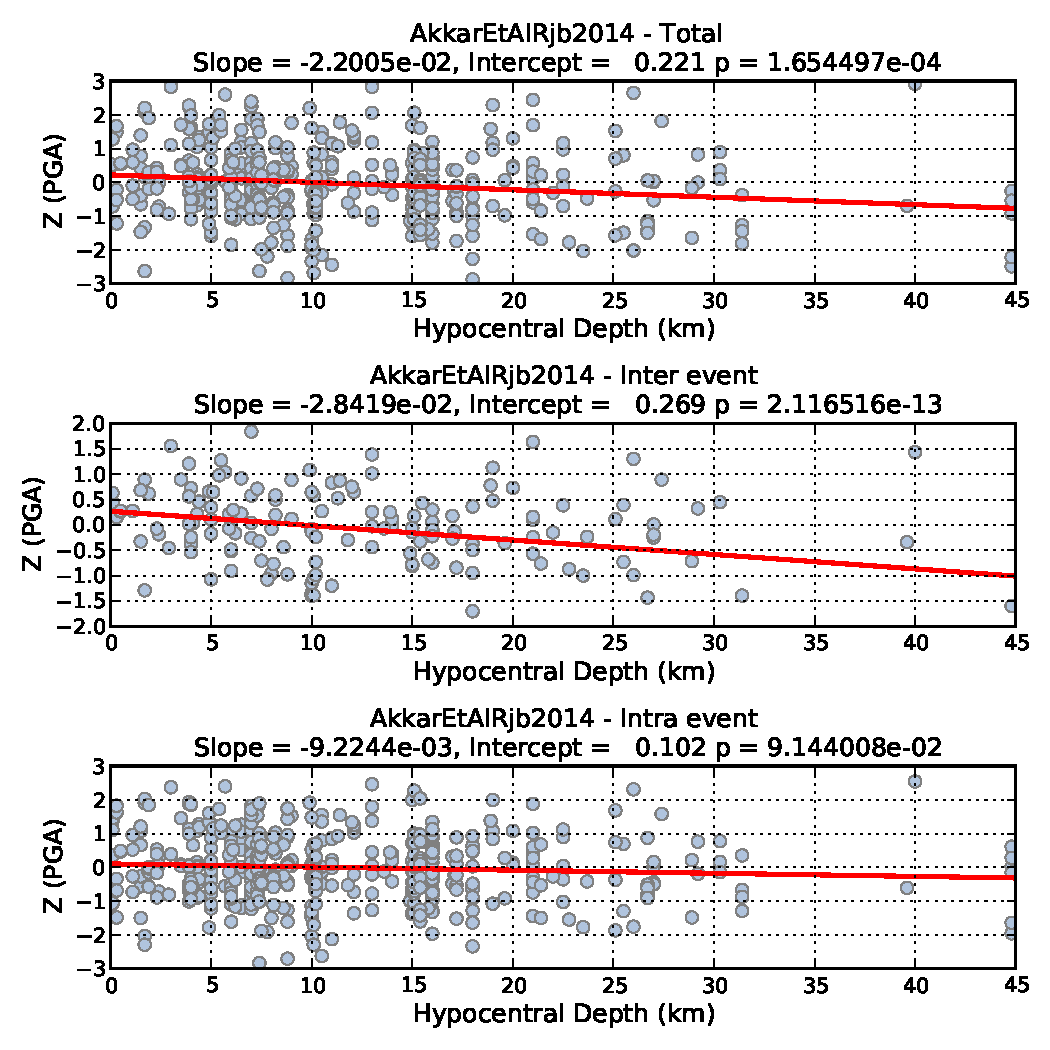
\includegraphics[width=\textwidth]{./figures/residuals/Akkar2014_HypoDepth_PGA.pdf}
      \caption{\textcite{Akkar_etal2014} model - PGA}
      \label{fig:pga_depth_akkar2014}
  \end{subfigure}
    \begin{subfigure}[b]{0.49\textwidth}
      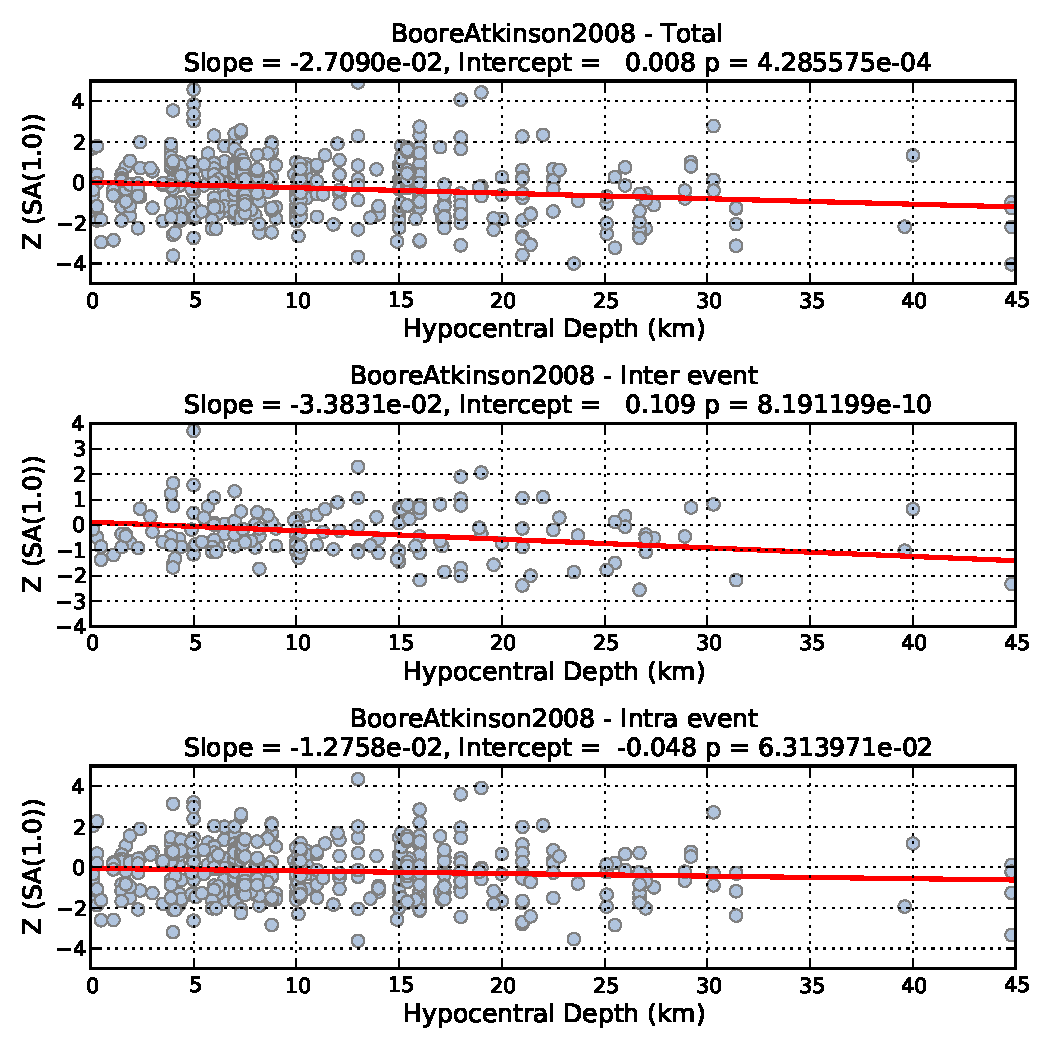
\includegraphics[width=\textwidth]{./figures/residuals/BA2008_HypoDepth_Sa1.pdf}
      \caption{\textcite{boore2008} model - $Sa \left( {1.0 s} \right)$}
      \label{fig:sa1_depth_ba2008}
  \end{subfigure}
      \begin{subfigure}[b]{0.49\textwidth}
      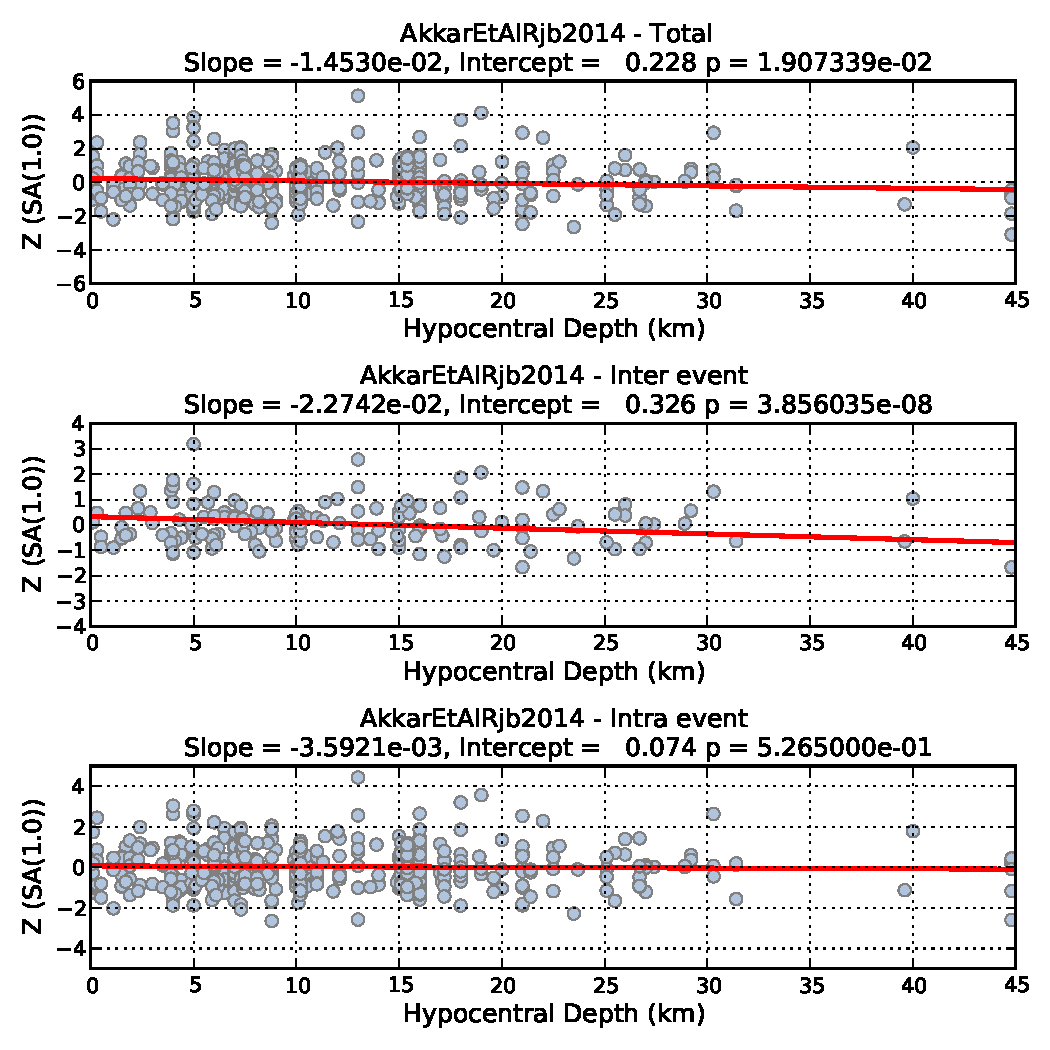
\includegraphics[width=\textwidth]{./figures/residuals/Akkar2014_HypoDepth_Sa1.pdf}
     \caption{\textcite{Akkar_etal2014} model - $Sa \left( {1.0 s} \right)$}
      \label{fig:sa1_depth_akkar2014}
  \end{subfigure}
  \caption{Residual trends with hypocentral depth for the observed PGA and $Sa \left( {1.0 s} \right)$ records}
  \label{fig:depth_resid}
\end{figure}

\section{Log-likelihood Approach \parencite{Scherbaum_etal2009}}
\label{sec:llh}

The analysis of GMPE residuals is critical in understanding where potential biases may exist when applying a particular ground motion model to a region, given a sufficiently robust set of observations. Ultimately in PSHA, however, it is necessary to make an inference as to whether or not the GMPE is suitable for application, and if so, how should these be weighted within the epistemic uncertainty analysis. The simple likelihood analysis presented so far in this chapter may not necessarily be sufficient for this purpose, as they may be biased by sample size and/or subjectivity on the criteria used to judge the fit of the model. One potential means of finding quantitative and objective measures by which the fit of GMPEs to a data set can be compared is via the use of information theory.

Consider the case of two models defined by continuous probability distributions $f \left( x \right)$ and $g \left( x \right)$ respectively. If model $f \left( x \right)$ is not known explicitly, but has been sampled $N$ times, such that the observation set is $\mathbf{x} = \left\{ {x_i} \right\}$ for $i = 1, \ldots, N$, then the likelihood of model $g \left( x \right)$ given the observations is defined as:

\begin{equation}
\mathcal{L}\left( {g | \mathbf{x}} \right) = \prod_{i=1}^{N} g \left( {x_i} \right)
\end{equation}

\noindent which for a measure independent of sample size becomes the average sample log-likelihood:

\begin{equation}
LLH = \langle \log_b \left( {\mathcal{L} \left( {g | \mathbf{x}} \right)} \right) \rangle = \frac{1}{N}\sum\limits_{i=1}^{N} \log_b \left( {g \left( {x_i} \right)} \right)
\end{equation}

\noindent where $b=2$ if considering information in ``bits''.

The close the two models the larger the corresponding log-likelihood. This concept can be applied to GMPEs, which are themselves probability distributions. If the set of observations is sampled from the model $f \left( x \right)$, in this case representing the ``true'' model, then the information loss that occurs by representing $f \left( x \right)$ by the model $g \left( x \right)$ is determined via the Kullback-Leibler distance:

\begin{equation}
D \left( {f, g} \right) = \int_{-\infty}^{\infty} f \left( x \right) \log_b \left( {\frac{f \left( x \right)}{g \left( x \right)}} \right) dx
\end{equation}

To compare the information loss for multiple GMPEs, given that the ``true'' model is unknown but that it is represented by $N$ samples, the model distance between the ``true'' model and the GMPE is represented by the negative average sample log-likelihood.

\textcite{Scherbaum_etal2009} provide a potential means of deriving weights for each model within a set of models using the average sample log-likelihood:  

\begin{equation}
w_l = \frac{2^{-LLH}}{\sum_{k=1}^{K}2 ^{-LLH}}
\end{equation}


To illustrate this we use the \verb=LLH= tool from the \verb=res= module. We consider the same four GMPEs and the same set of records. The \verb=LLH= analysis is run as follows:

\begin{python}[frame=single]
llh_1 = res.LLH(gmpe_list, imt_list)
llh_1.get_residuals(italy_db_clean)
 Run LLH analysis
llh_values, weights = llh_1.get_loglikelihood_values()
\end{python}

To view the $LLH$ values and weights, it is only necessary to do the following:

\begin{python}
for gmpe in gmpe_list:
    print "LLH(%s) = %12.6f Weight = %12.6f" %(gmpe,
                                               llh_values[gmpe],     
                                               weights[gmpe])
\end{python}

\noindent which, for the GMPEs and the strong motion database considered throughout this chapter, returns an output similar to that below:

\begin{verbatim}
LLH(BooreAtkinson2008) =     3.025793  Weight =     0.175937
LLH(AkkarBommer2010) =     2.559079  Weight =     0.243138
LLH(AkkarCagnan2010) =     2.366239  Weight =     0.277909
LLH(AkkarEtAlRjb2014) =     2.241463  Weight =     0.303015
\end{verbatim}

In this particular case it is, as expected, the \textcite{Akkar_etal2014} GMPE that provides the smallest average sample log-likelihood, and would therefore be assigned a greater weighting.

\section{Euclidean Distance Based Ranking \parencite{KaleAkkar2013}}
\label{sec:edr}

In an assessment of the log-likelihood ($LLH$) method, \textcite{KaleAkkar2013} indicate that the method may favour GMPEs with higher standard deviation values, largely due to the fact that outlier observations are predicted with higher probabilities in such models. As an alternative, they propose the Euclidean Distance-based Ranking (EDR). Consider a single observation ($a$) and its corresponding model estimate ($Y$), in this case the model is a Gaussian random variable with mean $\mu_Y$ and standard deviation $\sigma_Y$. The difference, $D$, between $a$ and $Y$ is defined as:

\begin{equation}
D = a - Y
\end{equation}
\noindent which is itself normally distributed with $\mu_D = a - \mu_Y$ and standard deviation $\sigma_D = \sigma_y$. The probability that the absolute value of $D$ is less than a specific estimate $d$ is therefore defined as:

\begin{eqnarray}
P \left( {|D| < d} \right) &=& P \left( {D < d} \right) - P \left( {D < -d} \right) \nonumber \\
 &=& \Phi \left( {\frac{d - \mu_D}{\sigma_D}} \right) - \Phi \left( {\frac{-d - \mu_D}{\sigma_D}} \right)
\end{eqnarray}

For discrete values of D, denoted by $d_j$, the occurrence probability of $d_j$ ($P \left( {d_j} \right)$) is described with a small bandwidth $dd$ around $d_j$, such that:

\begin{equation}
P \left( {|D| < |d_j|} \right) = P \left( {|D| < |d_j + \frac{dd}{2}|} \right) - P \left( {|D| < |d_j - \frac{dd}{2}|} \right)
\end{equation}

The total occurrence probability for a set of $|d_j|$ values is the modified Euclidean distance (MDE):

\begin{equation}
MDE_d = \sum_{j=1}^{n} |d_j| P \left( {|D| < |d_j|} \right)
\end{equation}

The modified Euclidean Distance ($MDE$) does not explicitly consider potential in the median value of the GMPE with respect to the observations.  To quantify the level of bias in the predictions of the median values a parameter $\kappa$ is introduced, which is the ratio of the total Euclidean distance between observed and expected median ground motions with respect the Euclidean Distance between the expected motions and the observed values corrected by a predictive model derived from a simple linear regression on the data. 

\begin{equation}
\kappa = \frac{\sum\limits_{i=1}^{N} \left( {a_i - Y_i} \right)^2}{\sum \limits_{i=1}^{N} \left( {a_i - Y_{c,i}} \right)^2}
\end{equation}

\noindent where $Y_{c,i} = Y_i - \left( {Y_{fit,i} - a_i} \right)$ and $Y_{fit,i}$ is the predicted value of the observation from a linear regression of $Y_i$ against $a_i$.

The sum of the modified Euclidean Distances represents the overall probability of the differences between the observed and estimated ground motion. Consequently a smaller sum of the $MDE$ values indicates a better representation of the ground motion from the predictive model. To eliminate the dependency on sample size the sum of the $MDE$ values is divided by the number of observations, to give the mean $MDE$. Finally to penalise to penalise predictive models displaying a larger bias in the median estimations, the mean $MDE$ is multiplied by $\kappa$. The final Euclidean Distance Ranking ($EDR$) or a GMPE with respect to the dataset is therefore calculated via:

\begin{equation}
EDR^2 = \kappa \times \frac{1}{N} \times \sum_{i=1}^{N} MDE_i^2
\end{equation}

To run an Euclidean distance-based ranking analysis for a database, the following process should be followed:

\begin{python}[frame=single]
# EDR analysis
edr1 = res.EDR(gmpe_list, imt_list)
edr1.get_residuals(italy_db_clean)
edr_values = edr1.get_edr_values()
\end{python}

The $EDR$ values and corresponding information can be viewed with the following:

\begin{python}
for gmpe in gmpe_list:
    print "EDR(%s) = %8.4f (sqrt(kappa) = %8.4f)" %(gmpe,
        edr_values[gmpe]["EDR"], edr_values[gmpe]["sqrt Kappa"])
\end{python}

\begin{verbatim}
EDR(BooreAtkinson2008) =   1.2163 (sqrt(kappa) =   1.1840)
EDR(AkkarBommer2010) =   1.0990 (sqrt(kappa) =   1.0609)
EDR(AkkarCagnan2010) =   1.3704 (sqrt(kappa) =   1.1308)
EDR(AkkarEtAlRjb2014) =   1.0956 (sqrt(kappa) =   1.0889)
\end{verbatim}

\section{Site Specific Analysis}
\label{sec:site}

Recalling from equation \ref{eq:gmpe_randeff}, the aleatory variability of the GMPE can be separated into two components: the intra-event residual($\delta_{E,j}$) and the inter-event residual ($\delta_{A,ij}$). When considering a single site with multiple ground motion records the total variability in the inter-event residual at the given site can be determined from:

\begin{equation}
\delta S2S_S = \frac{1}{N_{EQ}} \sum\limits_{j = 1}^{N_{EQ}} \delta_{A,ij}
\end{equation}

\noindent where $\delta S2S_S$ represents the average within-event residual at the station recorded from $N_{EQ}$ events. If there is minimal bias in the sub-set of single station records, this term should have a zero mean and a standard-deviation of $\phi_{S2S}$ \parencite{RodriguezMarek_etal2011}. Therefore the total aleatory variability ($\delta_{T,ij}$) can be decomposed into an average site-specific intra-event term and a residual variability, denoted by $\delta W_{o,ij}$:

\begin{equation}
\delta_{T,ij} = \delta_{E,j} + \delta S2S_S + \delta W_{o,ij}
\end{equation}

For a single station average within-event residual is a deterministic characteristic of the station. The ground motion variability for each station can then be computed by removing this term from the residuals. Taking the standard deviation of this term for each station returns the single-station standard deviation for the station ($\phi_{ss,s}$):

\begin{equation}
\phi_{ss,s} = \sqrt{\frac{\sum\limits_{j=1}^{N_{EQ}} \left( {\delta_{A,ij} - \delta S2S_S} \right)^2 }{N_{EQ} - 1}}
\end{equation}

For a subset of $N_{SITES}$ records within a database the total single-station standard deviation ($\phi_{ss}$) for the specific ground motion prediction equation can then be determined from:

\begin{equation}
\phi_{ss} = \sqrt{\frac{\sum\limits_{i=1}^{N_{SITES}} \sum\limits_{j=1}^{N_{EQ,i}} \left( {\delta_{A,ij} - \delta S2S_S} \right)^2}{\left( {\sum\limits_{i=1}^{N_{SITES}}} N_{EQ,i} \right) - 1}}
\end{equation}

\subsection{Single-Station $\sigma$ Example}

In this example we return to the full strong motion database to consider only sites that are associated with many records. To identify such sites a small function is found inside of the module \verb=strong_motion_selector=, which is named \verb=rank_sites_by_record_count=. This function will read an input database an return the identifier, name and number of records for each site in descending order of number of records. A threshold value can be input to limit the list of returned site information to just those sites with a number of records greater than or equal to the \verb=threshold= value. This is illustrated as follows:

\begin{python}
# Import the function
from smtk.strong_motion_selector import rank_sites_by_record_count
# Return the list of sites in our database containing
# more than 30 records
top_sites = rank_sites_by_record_count(db1, threshold=30)
for site_id in top_sites.keys():
    print "Site ID: %s   Name: %s  Number of Records: %s" %(
        site_id,
        top_sites[site_id]["Name"],
        top_sites[site_id]["Count"])
\end{python}

\noindent In the present example this returns the information shown:

\begin{verbatim}
Site ID: 155    Name: 5401  Number of Records: 60
Site ID: 134    Name: 3502  Number of Records: 55
Site ID: 183    Name: 9906  Number of Records: 49
Site ID: 229    Name: 1201  Number of Records: 45
Site ID: 2322   Name: 4802  Number of Records: 44
Site ID: 187    Name: 9901  Number of Records: 44
Site ID: 153    Name: 1701  Number of Records: 40
Site ID: 184    Name: 9907  Number of Records: 39
Site ID: 182    Name: 9902  Number of Records: 39
Site ID: 194    Name: 9904  Number of Records: 39
Site ID: 188    Name: 1401  Number of Records: 35
Site ID: 105    Name: 2002  Number of Records: 33
Site ID: 149    Name: 3401  Number of Records: 32
Site ID: 2466   Name: 2007  Number of Records: 31
Site ID: 139    Name: 1001  Number of Records: 31
Site ID: 2591   Name: 2501  Number of Records: 30
\end{verbatim}

This returns 16 sites for which more than 30 records exist in our database. The first step is to get the residual information for the sites. This can be done using the function in the \verb=res= module called \verb=SingleStationAnalysis=. This function requires as input the list of GMPE's used for the residual analysis and the list of intensity measures. In this case we consider only the \textcite{Akkar_etal2014} GMPE using $PGA$ and $Sa \left( {1.0 s} \right)$.

\begin{python}
# Consider the AkkarEtAlRjb2014 GMPE with PGA, Sa (0.2), Sa(1.0)
gmpe_list = ["AkkarEtAlRjb2014"]
imt_list = ["PGA", "SA(0.2)", "SA(1.0)"]
# Get the residuals for the site
site_ids = top_sites.keys()
ssa1 = res.SingleStationAnalysis(top_sites.keys(),
                                 gmpe_list,
                                 imt_list)
ssa1.get_site_residuals(db1)
\end{python}

The \verb=SingleStationAnalysis= module is instantiated with a list of station IDs, a list of GMPEs and a list of the intensity measure types. The analysis is then run on the input database.

Two visualisation tools are available in the \verb=rspl= modules: \verb=ResidualsWithSite= and \verb=IntraEventResidualWithSite=. The former creates plots of normalised total-, inter- and intra-event residual for a a set of sites, given a particular GMPE and intensity measure type. For example, using the \textcite{Akkar_etal2014}, the normalised residuals for the stations listed previously are shown can be calculated for PGA and $Sa \left( {1.0 s} \right)$ using the following, and the results may be similar to those shown in Figure \ref{fig:ssa_normalised_residuals}:

\begin{python}
rspl.ResidualWithSite(ssa1,
                      "AkkarEtAlRjb2014",
                      "PGA",
                      figure_size=(7,7),
                      filename="path/to/image.pdf",
                      filetype="pdf")
rspl.ResidualWithSite(ssa1,
                      "AkkarEtAlRjb2014",
                      "SA(1.0)",
                      figure_size=(7,7),
                      filename="path/to/image.pdf",
                      filetype="pdf")
\end{python}

\begin{figure}[htb]
  \centering
  \begin{subfigure}[b]{0.49\textwidth}
      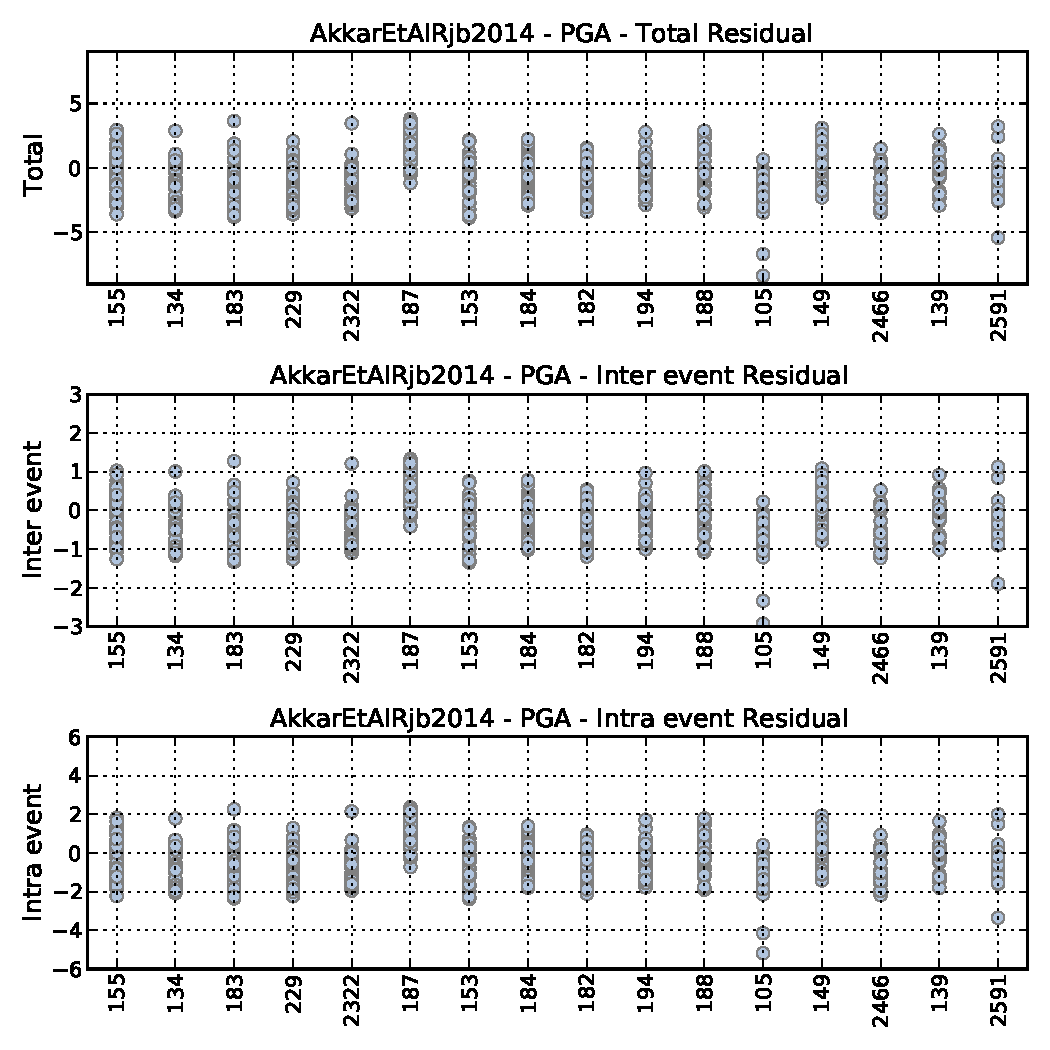
\includegraphics[width=\textwidth]{./figures/residuals/Single_Station_Residuals_PGA.pdf}
      \caption{PGA}
      \label{fig:ssa_residual_pga}
  \end{subfigure}
    \begin{subfigure}[b]{0.49\textwidth}
      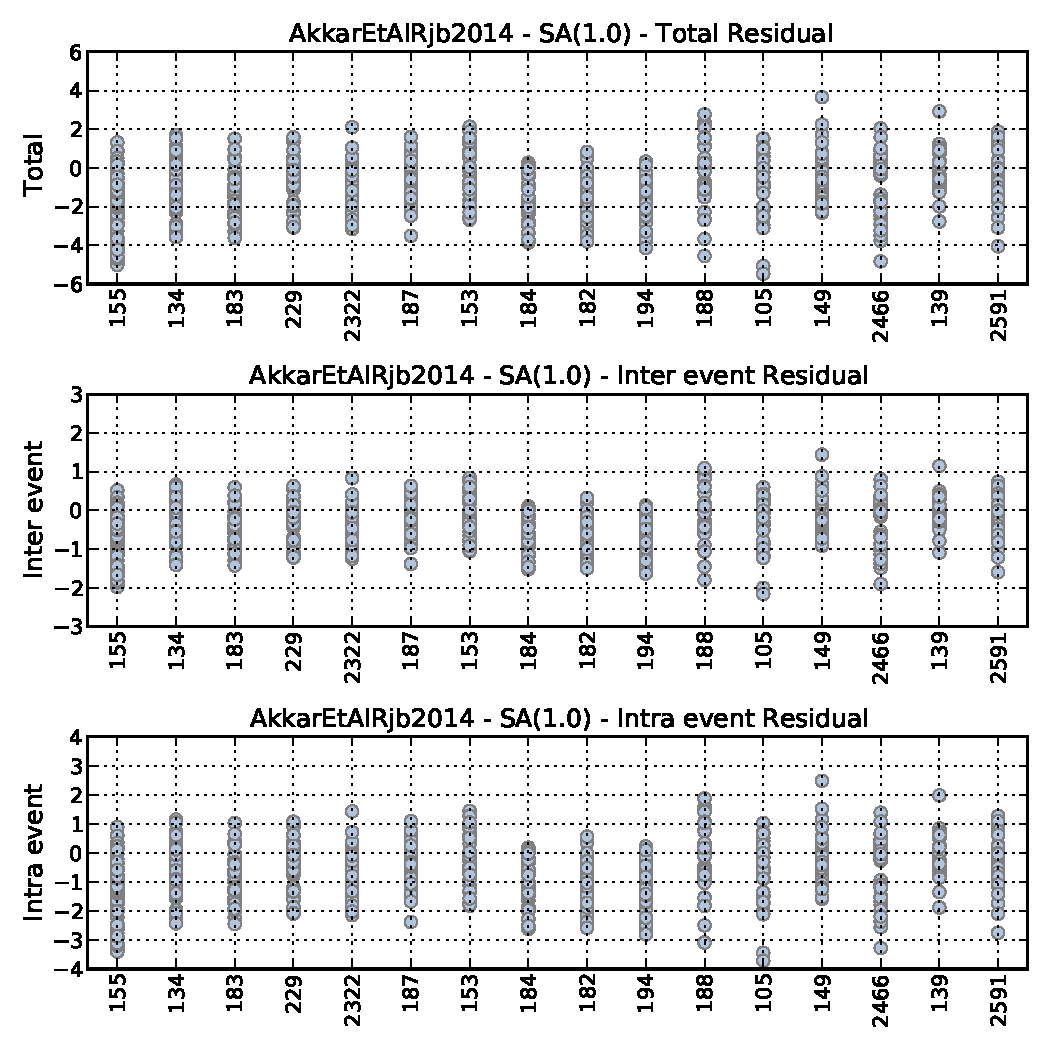
\includegraphics[width=\textwidth]{./figures/residuals/Single_Station_Residuals_Sa1.pdf}
      \caption{$Sa \left( {1.0s} \right)$}
      \label{fig:ssa_residual_sa1}
  \end{subfigure}
  \caption{PGA and $Sa \left( {1.0 s} \right)$ Residuals for each station}
  \label{fig:ssa_normalised_residuals}
\end{figure}

To view the distribution of $\delta S2S_S$ and $\delta W_{o,ij}$ for each site, and calculate the variability in the average within-event residual to return $\phi_{S2S}$ and $\phi_{SS}$ for the corresponding GMPE and intensity measures, the \verb=IntraEventResidualWithSite= tool is used. For the \textcite{Akkar_etal2014} GMPE and the decomposition of the intra-event residual for PGA and $Sa \left( {1.0s} \right)$ is run as follows, and would produce results similar to those shown in Figure \ref{fig:ssa_intra_decom}:

\begin{python}
rspl.IntraEventResidualWithSite(ssa1,
                                "AkkarEtAlRjb2014",
                                "PGA",
                                figure_size=(7,7),
                                filename="path/to/image.pdf",
                                filetype="pdf")
                                
rspl.IntraEventResidualWithSite(ssa1,
                                "AkkarEtAlRjb2014",
                                "SA(1.0)",
                                figure_size=(7,7),
                                filename="path/to/image.pdf",
                                filetype="pdf")
\end{python}


\begin{figure}[htb]
  \centering
  \begin{subfigure}[b]{0.49\textwidth}
      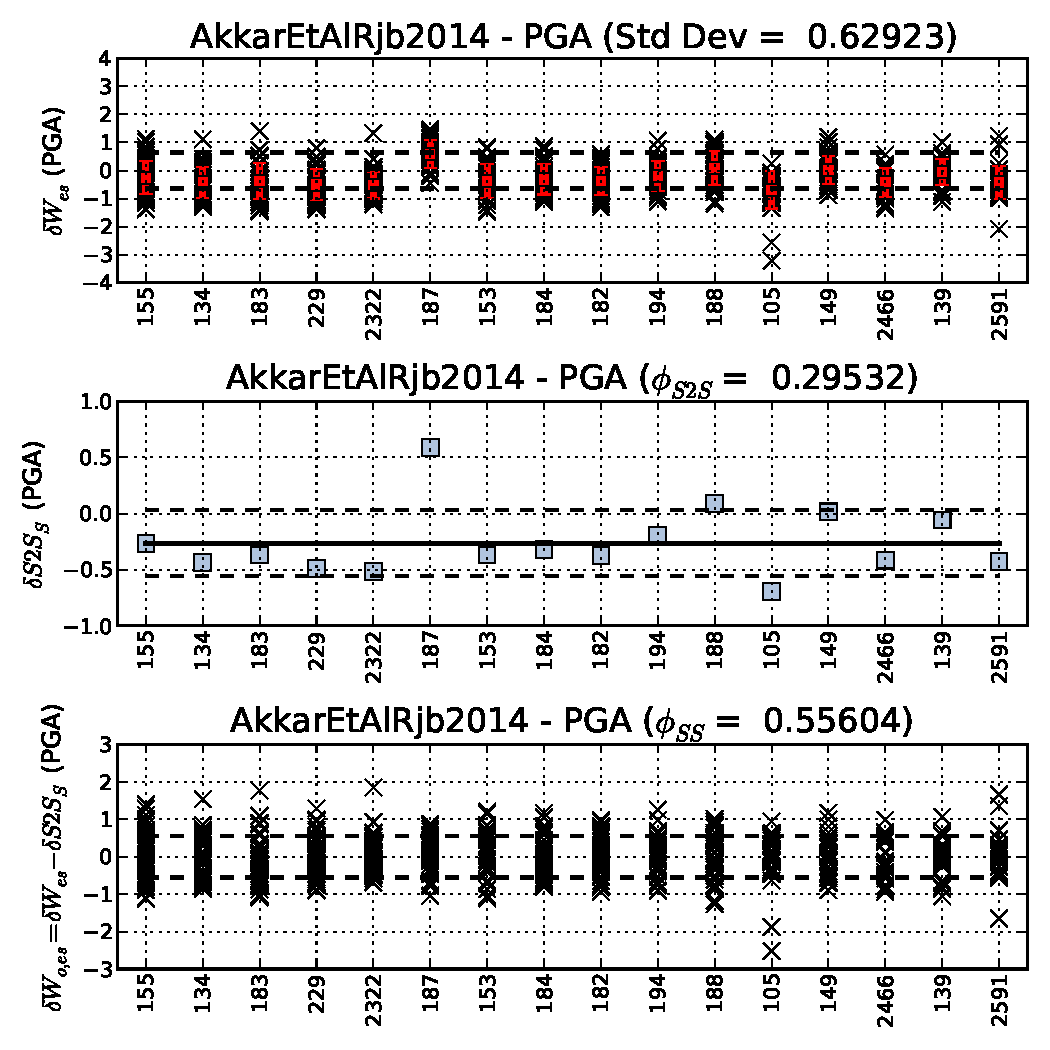
\includegraphics[width=\textwidth]{./figures/residuals/Single_Station_IntraEvent_PGA.pdf}
      \caption{PGA}
      \label{fig:ssa_intra_pga}
  \end{subfigure}
    \begin{subfigure}[b]{0.49\textwidth}
      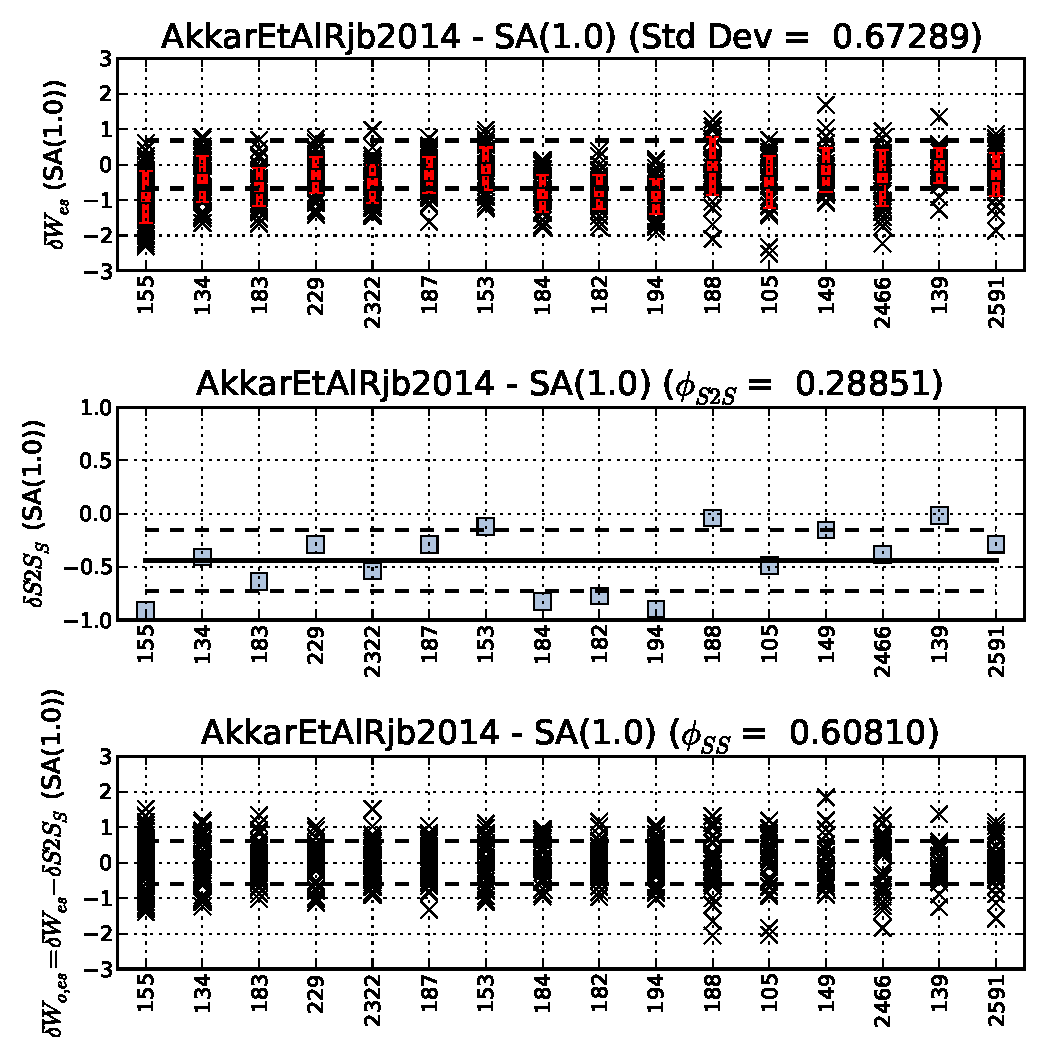
\includegraphics[width=\textwidth]{./figures/residuals/Single_Station_IntraEvent_Sa1.pdf}
      \caption{$Sa \left( {1.0s} \right)$}
      \label{fig:ssa_intra_sa1}
  \end{subfigure}
  \caption{Decomposition of Intra-event residuals for PGA and $Sa \left( {1.0 s} \right)$ for each station using the \cite{Akkar_etal2014} GMPE}
  \label{fig:ssa_intra_decom}
\end{figure}

In Figure \ref{fig:ssa_intra_decom} the analysis is broken down into three components, similar to that shown in Figure 5 of \textcite{RodriguezMarek_etal2011}. The top figure for each plot shows the observed intra-event residual for each site, \textbf{not} normalised by the intra-event standard deviation $\sigma$. Taking the standard deviation of these residual values should, in theory, approximately equal the intra-event standard deviation for the GMPE. In the present case the original GMPE $\sigma$ for PGA was equal to 0.6201, and for $Sa \left( {1.0s} \right)$ it was equal 0.6787. In the top graph in Figure \ref{fig:ssa_intra_decom} the total standard deviation of all the non-normalised intra-event residuals is very close to the GMPE $\sigma$. In the middle plot we see the average within-event residual for each station. In this example we observe that these values do not have a zero mean, suggesting a potential bias in the sample of stations. All 16 stations come from the same region (Turkey) of the data set. The standard deviation of the average within-event residuals for the subset of stations ($\phi_{S2S}$) is shown. Finally, in the bottom figure we see the distribution residual variabilities (i.e. $\delta_{A,ij} - \delta S2S_S$) for each of the stations. The standard deviation of these terms represents the single-station standard deviation ($\phi_{SS}$) of the whole model. This term should usually, but may not always, be smaller than the intra-event residual of the GMPE. This value is an estimate of the non-ergodic standard deviation for the GMPE. 



